\chapter{Suppl\texorpdfstring{ementary}{.} material for Chap\texorpdfstring{ter}{.}
\getrefnumber{ch:Integration}}\label{ch:SupplIntegration}
%\chaptermark{Supplementary material for \getrefnumber{ch:Integration}}


\begin{figure}
    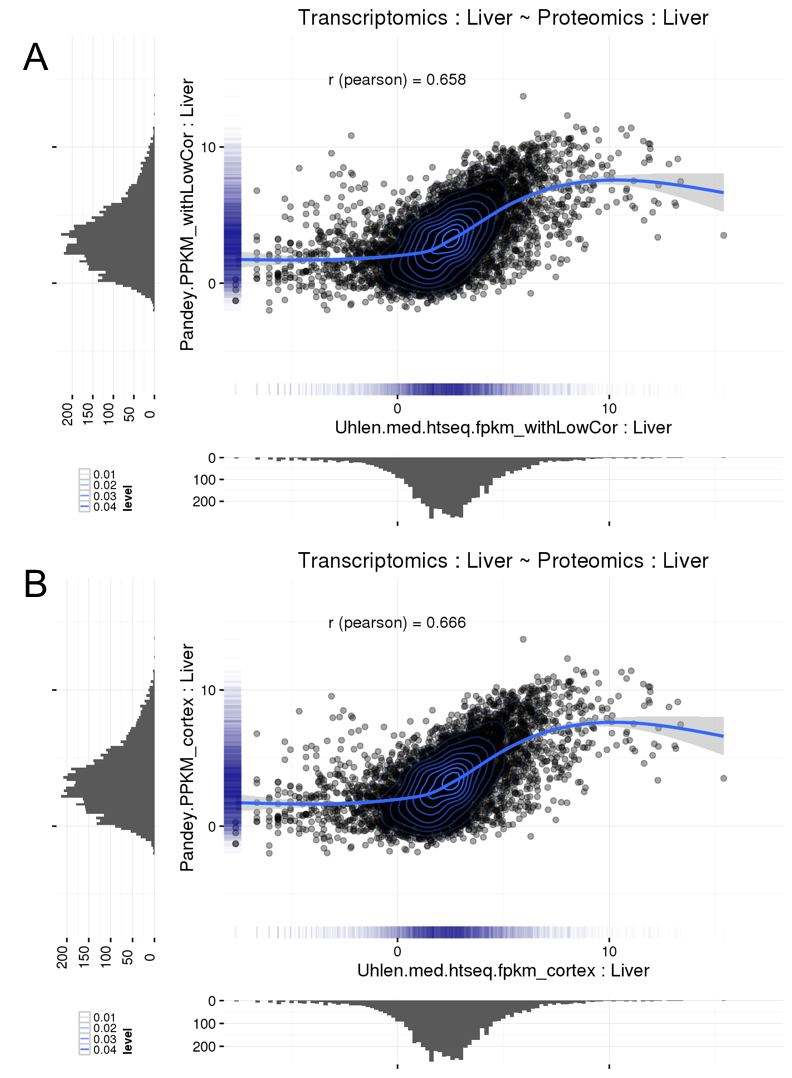
\includegraphics[scale=0.75]{integration/LiverScat}\centering
    \caption[Scatter plot between transcriptomic and proteomic
    for Liver]{\label{fig:ScatterPlotLiver}\textbf{Scatter plot between
    transcriptomic (x-axis) and proteomic (y-axis) for Liver}\\
    A| with the anticorrelated \mRNAs\ B| without the anticorrelated \mRNAs}
\end{figure}


\begin{figure}
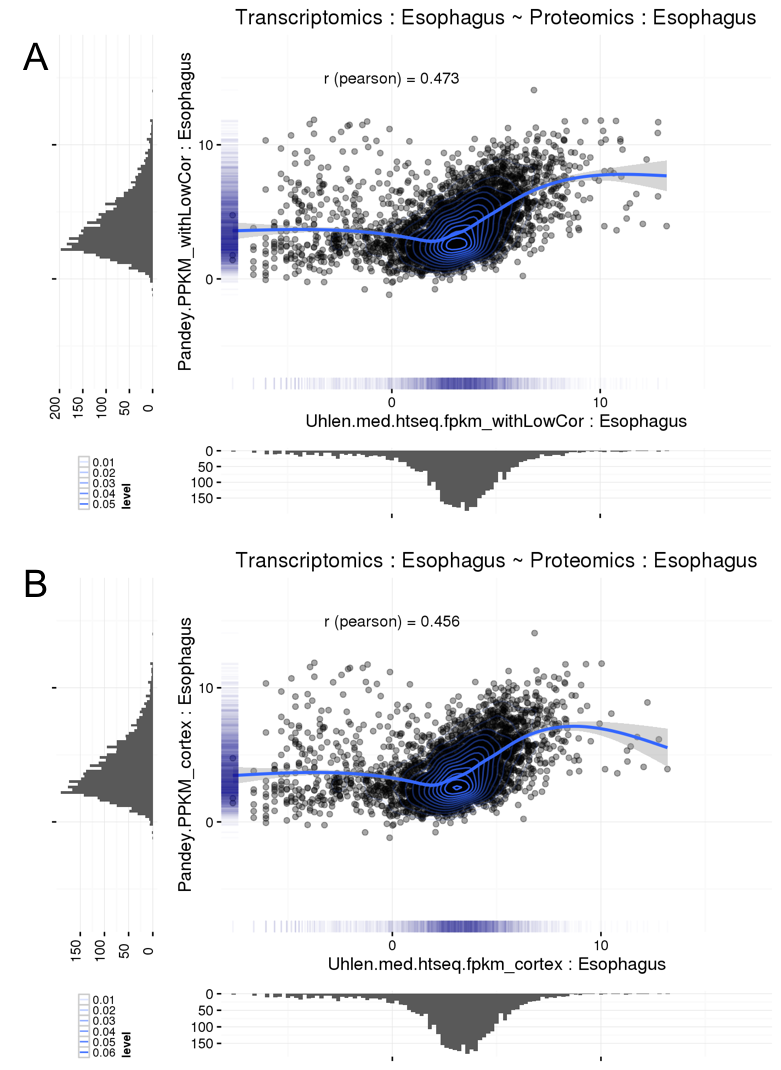
\includegraphics[scale=0.75]{integration/OesophagusScat}\centering
    \caption[Scatter plot between transcriptomic and
    proteomic for Oesophagus]{\label{fig:ScatterPlotOesophagus}\textbf{Scatter plot between
    transcriptomic (x-axis) and  proteomic (y-axis) for Oesophagus}\\
    A| with the anticorrelated \mRNAs\ B| without the anticorrelated \mRNAs}
\end{figure}


\begin{figure}
    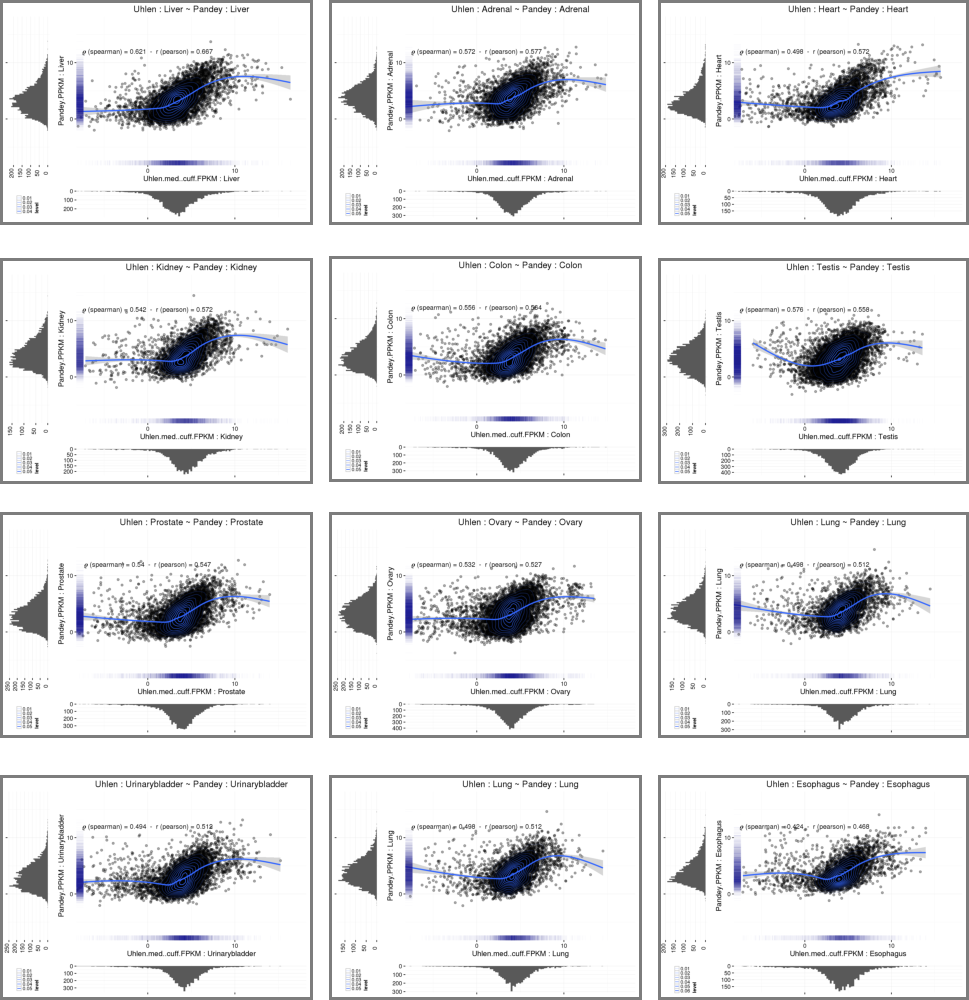
\includegraphics[scale=0.9]{integration/scatterplots.pdf}\centering
    \caption[Scatter plot between transcriptomic and
    proteomic for all tissues]{\label{fig:ScatterPlotAll}\textbf{Scatter plot between
    transcriptomic (x-axis) and  proteomic (y-axis) for all the tissues}}
\end{figure}


\begin{figure}%[!htbp]
    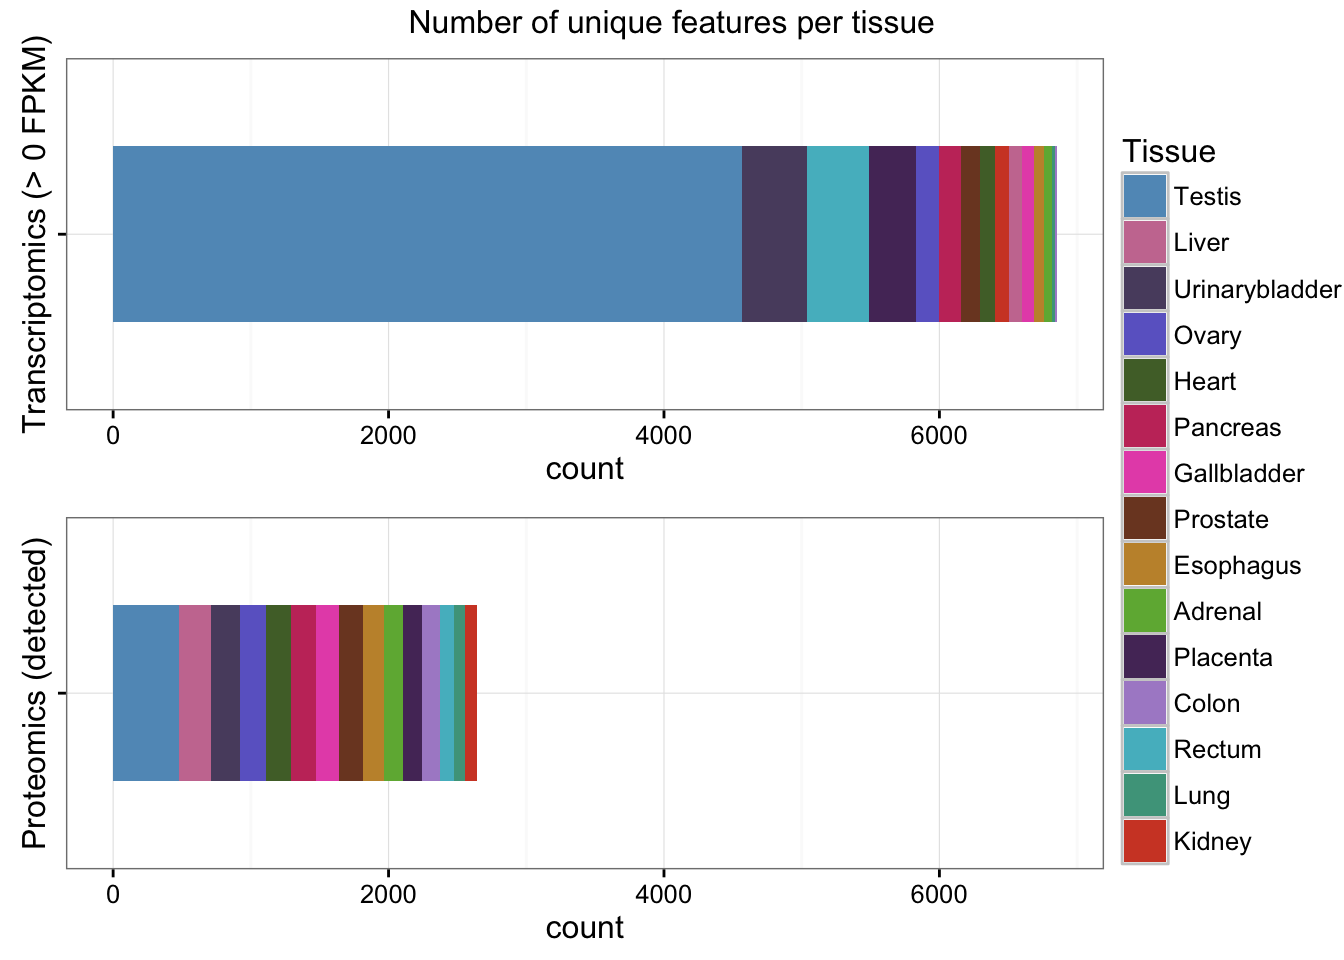
\includegraphics[scale=0.30]{integration/barPlotunique0nb}\centering
    \caption[Number of \mRNAs\ and proteins detected  only in one
    unique tissue]{\label{fig:barPlotunique0nb}\textbf{Number of
    \mRNAs\ (top) and proteins (bottom)
    that have been detected and quantified (\textgreater\ 0 \gls{FPKM} for \mRNA\
    and for proteins).}}
\end{figure}

\begin{figure}%[!htbp]
    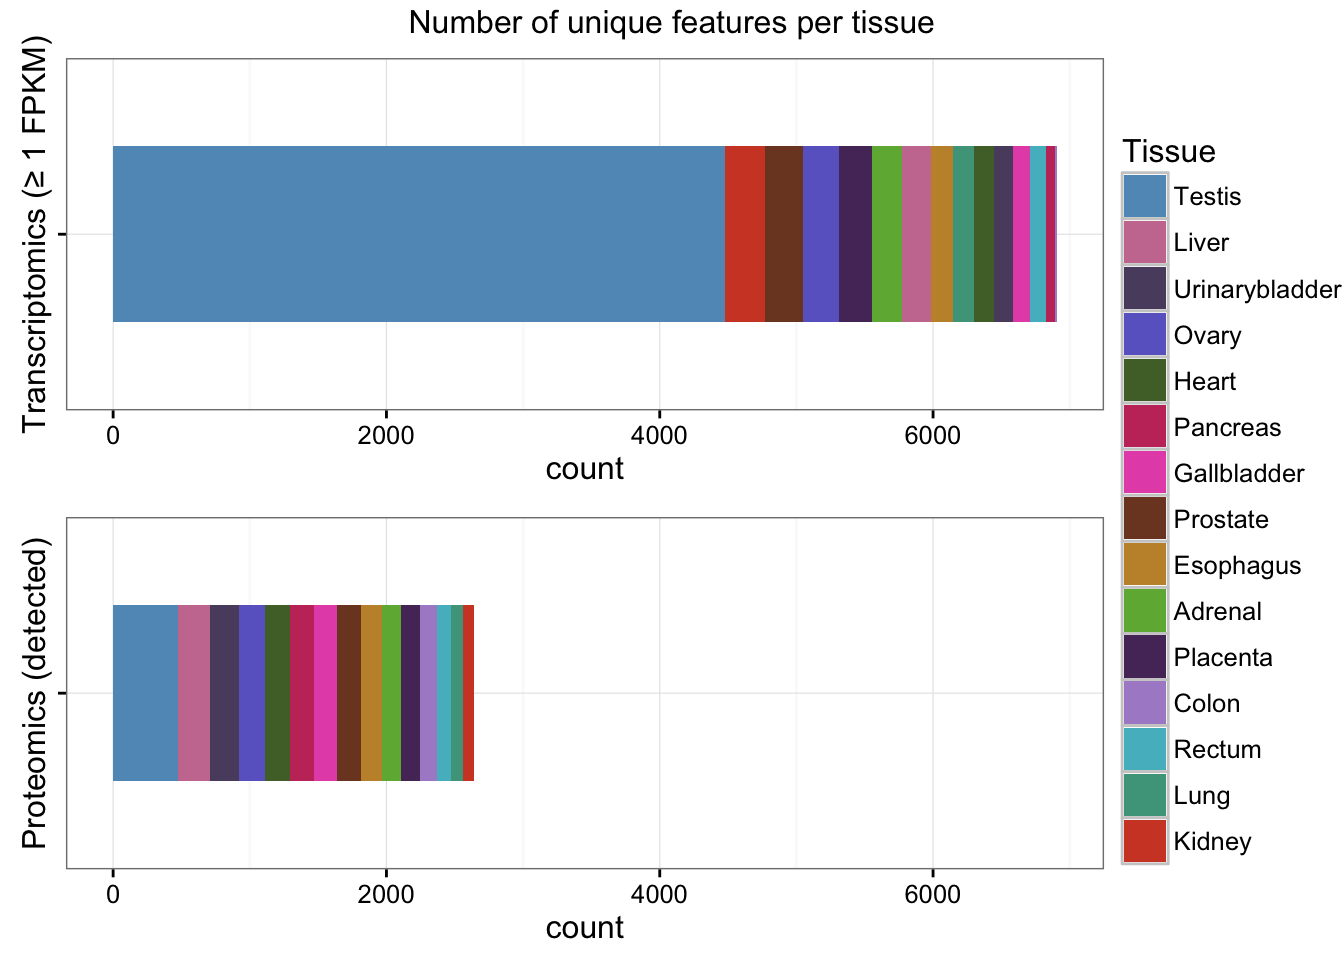
\includegraphics[scale=0.30]{integration/barPlotunique1nb}\centering
    \caption[Number of \mRNAs\ (\geq\ 1 \gls{FPKM})
    and proteins detected (at specific thresholds) only in one unique
    tissue]{\label{fig:barPlotunique1nb}\textbf{Number of
    \mRNAs\ (top) and proteins (bottom)
    that have been detected and quantified (\geq\ 1 \gls{FPKM} for \mRNA\;
    \textgreater\ 0 for proteins).} While some tissue can have consistently a higher
    specificity at proteomic and transcriptomic level, it is not true for all.}
\end{figure}



\begin{figure}%[!htbp]
    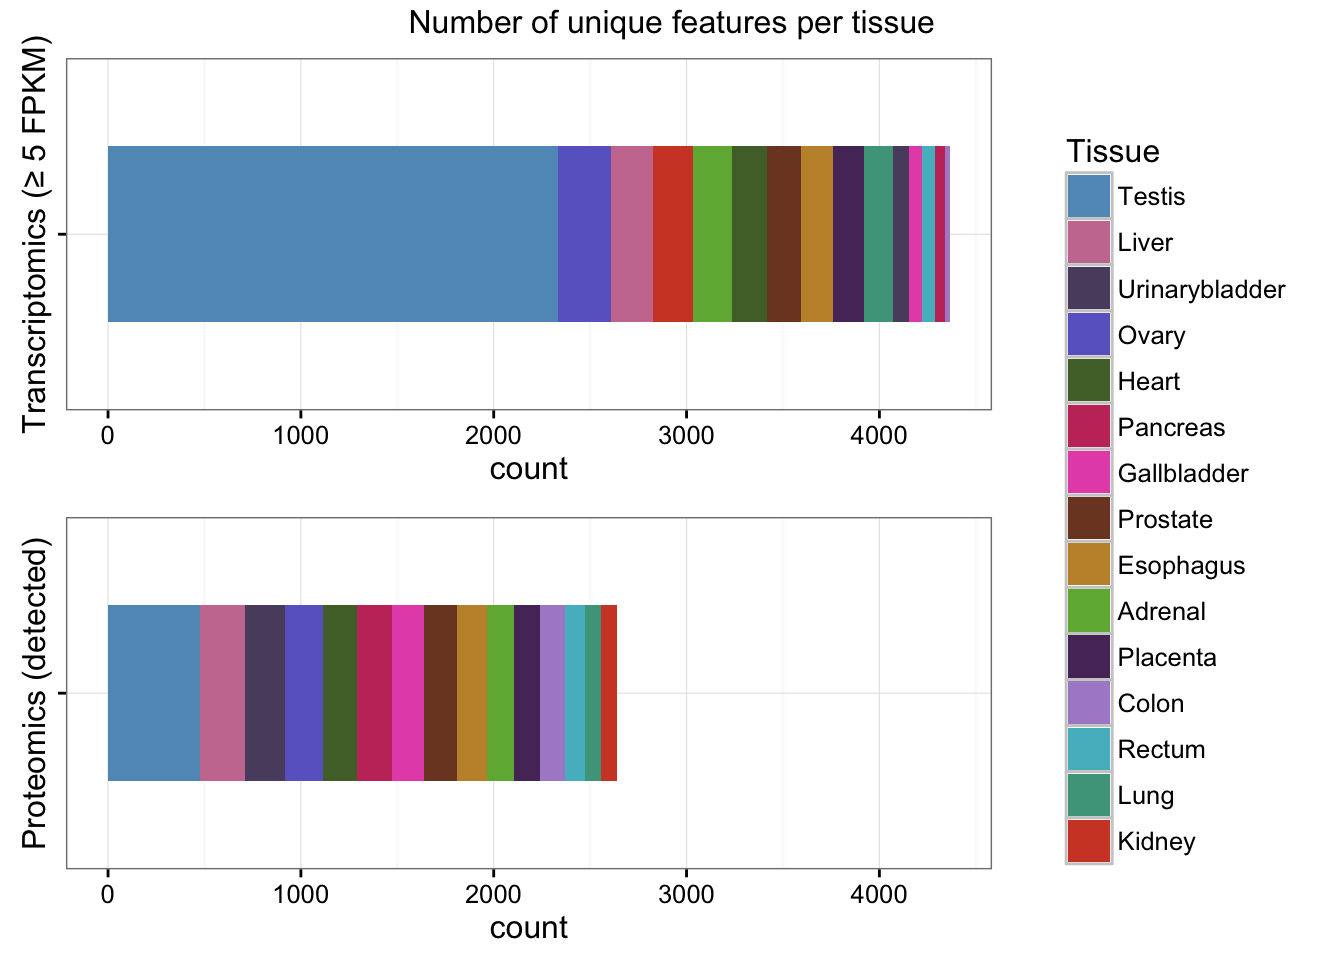
\includegraphics[scale=0.30]{integration/barPlotunique5nb}\centering
    \caption[Number of \mRNAs\ (\geq\ 5 \glspl{FPKM}) and proteins detected
    (at specific thresholds) only in one unique
    tissue]{\label{fig:barPlotunique5nb}\textbf{Number of \mRNAs\ (top)
    and proteins (bottom) that have been detected and quantified
    (\geq\ 5 \glspl{FPKM} for \mRNA\; \textgreater\ 0 for proteins).}}
\end{figure}


\begin{figure}[!htbp]
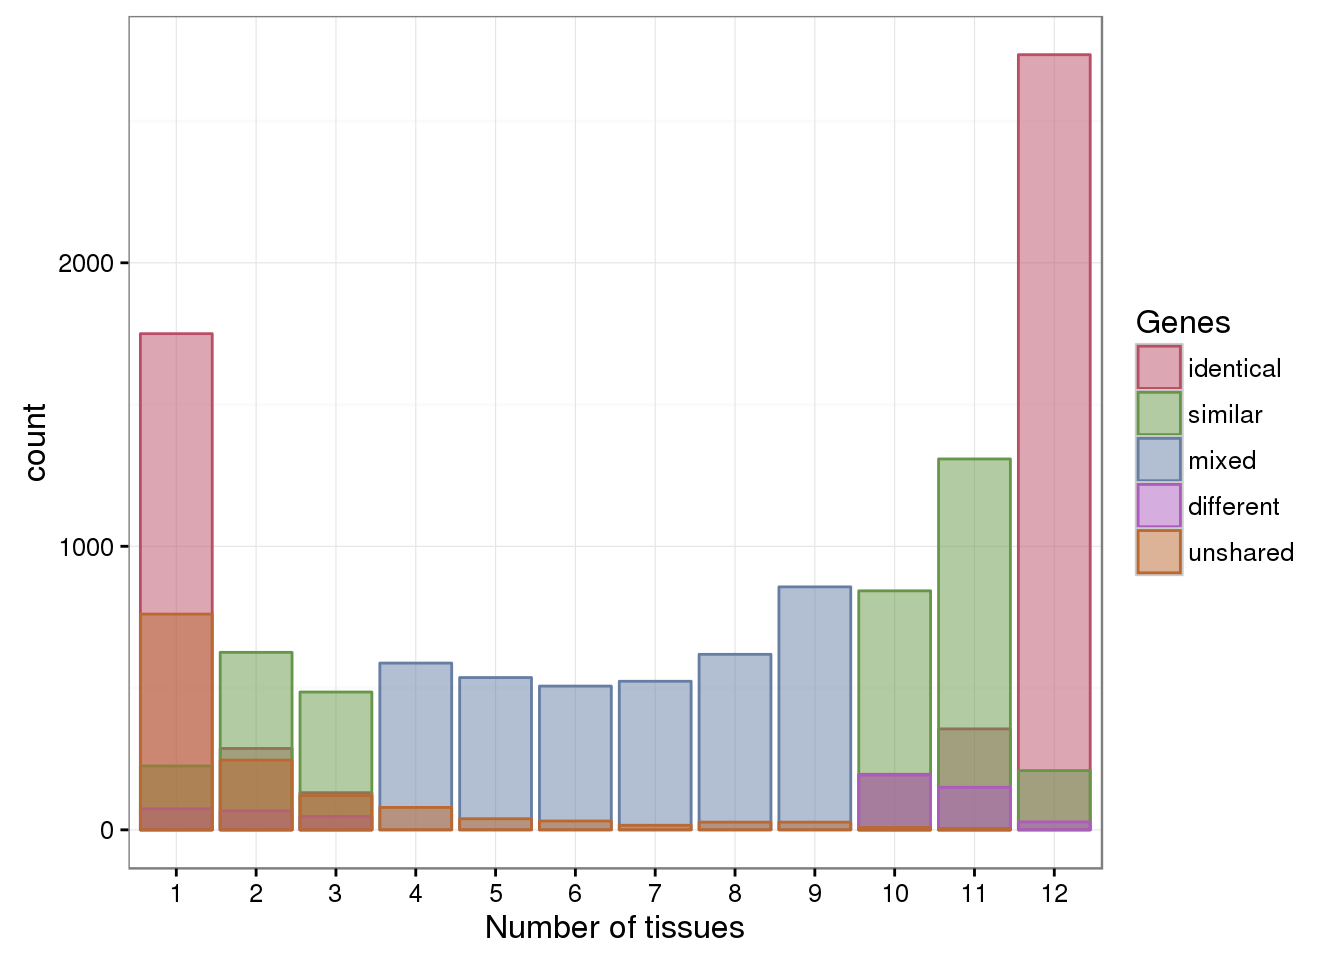
\includegraphics[scale=1]{integration/GtexUhlenAnnoBreadth}
\caption[placeHold]{\label{fig:breadthColGtexUhlen}\textbf{placeHold}}
\end{figure}




\clearpage
\thispagestyle{plain}
\small


\begin{landscape}
    \begin{longtable}{@{}llllll@{}}%[]%\centering
    \caption{Found proteins without a counterpart in the transcriptomic data}\label{tab:protNoTrans}\\
\toprule
Set & Ensembl Gene ID & Gene name & Biotype & Description & \begin{tabular}[c]{@{}l@{}}Source and \\ Accessing number\end{tabular} \\ \midrule
a, b, c, d & ENSG00000173349 & SFT2D3 & p.\ coding & SFT2 domain containing 3 & \begin{tabular}[c]{@{}l@{}}HGNC Symbol \\ Acc: 28767\end{tabular} \\
a, b & ENSG00000198788 & MUC2 & \begin{tabular}[c]{@{}l@{}}processed\\ transcript\end{tabular} & \begin{tabular}[c]{@{}l@{}}mucin 2, \\ oligomeric mucus/gel-forming\end{tabular} & \begin{tabular}[c]{@{}l@{}}HGNC Symbol\\ Acc: 7512\end{tabular} \\
a, b, c, d & ENSG00000223953 & C1QTNF5 & p.\ coding & \begin{tabular}[c]{@{}l@{}}C1q and tumor necrosis\\ factor related protein 5\end{tabular} & \begin{tabular}[c]{@{}l@{}}HGNC Symbol\\ Acc:14344\end{tabular} \\
a, b & ENSG00000256453 & DND1 & p.\ coding & \begin{tabular}[c]{@{}l@{}}DND microRNA-mediated \\ repression inhibitor\end{tabular} & \begin{tabular}[c]{@{}l@{}}HGNC Symbol\\ Acc:23799\end{tabular} \\
a, b, c, d & ENSG00000262664 & OVCA2 & p.\ coding & \begin{tabular}[c]{@{}l@{}}ovarian tumor suppressor\\ candidate 2\end{tabular} & \begin{tabular}[c]{@{}l@{}}HGNC Symbol\\ Acc:24203\end{tabular} \\
b & ENSG00000163157 & TMOD4 & p.\ coding & tropomodulin 4 (muscle) & \begin{tabular}[c]{@{}l@{}}HGNC Symbol\\ Acc:11874\end{tabular} \\
b & ENSG00000203618 & GP1BB & p.\ coding & \begin{tabular}[c]{@{}l@{}}glycoprotein Ib (platelet), \\ beta polypeptide\end{tabular} & \begin{tabular}[c]{@{}l@{}}HGNC Symbol\\ Acc:4440\end{tabular} \\
b & ENSG00000251322 & SHANK3 & \begin{tabular}[c]{@{}l@{}}processed\\ transcript\end{tabular} & \begin{tabular}[c]{@{}l@{}}SH3 and \\ multiple ankyrin repeat domains 3\end{tabular} & \begin{tabular}[c]{@{}l@{}}HGNC Symbol\\ Acc:14294\end{tabular} \\
c, d & ENSG00000105371 & ICAM4 & p.\ coding & \begin{tabular}[c]{@{}l@{}}intercellular adhesion molecule 4 \\ (Landsteiner-Wiener blood group)\end{tabular} & \begin{tabular}[c]{@{}l@{}}HGNC Symbol\\ Acc:5347\end{tabular} \\
c & ENSG00000164708 & PGAM2 & p.\ coding & phosphoglycerate mutase 2 (muscle) & \begin{tabular}[c]{@{}l@{}}HGNC Symbol \\ Acc:8889\end{tabular} \\
c, d & ENSG00000181404 & XXyac-YRM2039.2 & \begin{tabular}[c]{@{}l@{}}unprocesssed\\ pseudogene\end{tabular} &  &  \\
c, d & ENSG00000183336 & BOLA2 & p.\ coding & bolA family member 2 & \begin{tabular}[c]{@{}l@{}}HGNC Symbol\\ Acc:29488\end{tabular} \\
c & ENSG00000196101 & HLA-DRB3 & p.\ coding & \begin{tabular}[c]{@{}l@{}}major histocompatibility complex, \\ class II, DR beta 3\end{tabular} & \begin{tabular}[c]{@{}l@{}}HGNC Symbol\\ Acc:4951\end{tabular} \\
c & ENSG00000203618 & GP1BB &  & \begin{tabular}[c]{@{}l@{}}glycoprotein Ib (platelet), \\ beta polypeptide\end{tabular} & \begin{tabular}[c]{@{}l@{}}HGNC Symbol\\ Acc:4440\end{tabular} \\
c, d & ENSG00000206203 & TSSK2 & p.\ coding & testis-specific serine kinase 2 & \begin{tabular}[c]{@{}l@{}}HGNC Symbol\\ Acc:1140\end{tabular} \\
c, d & \begin{tabular}[c]{@{}c@{}}ENSG00000206240,\\ ENSG00000206306\end{tabular} & HLA-DRB1 & p.\ coding & \begin{tabular}[c]{@{}l@{}}major histocompatibility complex, \\ class II, DR beta 1\end{tabular} & \begin{tabular}[c]{@{}l@{}}HGNC Symbol\\ Acc:4948\end{tabular} \\
c, d & ENSG00000206305 & HLA-DQA1 &  & \begin{tabular}[c]{@{}l@{}}major histocompatibility complex,\\ class II, DQ alpha 1\end{tabular} & \begin{tabular}[c]{@{}l@{}}HGNC Symbol\\ Acc:4942\end{tabular} \\
c, d & \begin{tabular}[c]{@{}c@{}}ENSG00000206450,\\ ENSG00000223532\end{tabular} & HLA-B & p.\ coding & \begin{tabular}[c]{@{}l@{}}major histocompatibility complex, \\ class I, B\end{tabular} & \begin{tabular}[c]{@{}l@{}}HGNC Symbol \\ Acc:4932\end{tabular} \\
c, d & ENSG00000225691 & HLA-C & p.\ coding & \begin{tabular}[c]{@{}l@{}}major histocompatibility complex, \\ class I, C\end{tabular} & \begin{tabular}[c]{@{}l@{}}HGNC Symbol\\ Acc:4933\end{tabular} \\
c, d & \begin{tabular}[c]{@{}c@{}}ENSG00000206505,\\ ENSG00000224320,\\ ENSG00000227715,\\ ENSG00000235657,\\ ENSG00000223980,\\ ENSG00000229215\end{tabular} & HLA-A & p.\ coding & \begin{tabular}[c]{@{}l@{}}major histocompatibility complex,\\ class I, A\end{tabular} & \begin{tabular}[c]{@{}l@{}}HGNC Symbol\\ Acc:4931\end{tabular} \\
c, d & ENSG00000211594 & IGKJ4 & IG J gene & immunoglobulin kappa joining 4 & \begin{tabular}[c]{@{}l@{}}HGNC Symbol\\ Acc:5722\end{tabular} \\
c, d & ENSG00000211595 & IGKJ3 & IG J gene & immunoglobulin kappa joining 3 & \begin{tabular}[c]{@{}l@{}}HGNC Symbol\\ Acc:5721\end{tabular} \\
c & ENSG00000213402 & PTPRCAP & p.\ coding & \begin{tabular}[c]{@{}l@{}}protein tyrosine phosphatase,\\ receptor type, C-associated protein\end{tabular} & \begin{tabular}[c]{@{}l@{}}HGNC Symbol\\ Acc:9667\end{tabular} \\
c & ENSG00000215695 & RSC1A1 & p.\ coding & \begin{tabular}[c]{@{}l@{}}regulatory solute carrier protein, \\ family 1, member 1\end{tabular} & \begin{tabular}[c]{@{}l@{}}HGNC Symbol\\ Acc:10458\end{tabular} \\
c, d & ENSG00000227357 & HLA-DRB4 & p.\ coding & \begin{tabular}[c]{@{}l@{}}major histocompatibility complex, \\ class II, DR beta 4\end{tabular} & \begin{tabular}[c]{@{}l@{}}HGNC Symbol\\ Acc:4952\end{tabular} \\
c, d & ENSG00000231021 & HLA-DRB4 & p.\ coding & \begin{tabular}[c]{@{}l@{}}major histocompatibility complex,\\ class II, DR beta 4\end{tabular} & \begin{tabular}[c]{@{}l@{}}RefSeq mRNA\\ Acc:NM\_021983\end{tabular} \\
c, d & ENSG00000231286 & HLA-DQB1 & p.\ coding & \begin{tabular}[c]{@{}l@{}}major histocompatibility complex, \\ class II, DQ beta 1\end{tabular} & \begin{tabular}[c]{@{}l@{}}HGNC Symbol\\ Acc:4944\end{tabular} \\
c, d & ENSG00000231679 & HLA-DRB3 & p.\ coding & \begin{tabular}[c]{@{}l@{}}major histocompatibility complex,\\ class II, DR beta 3\end{tabular} & \begin{tabular}[c]{@{}l@{}}RefSeq mRNA\\ Acc:NM\_022555\end{tabular} \\
c, d & ENSG00000256453 & DND1 & p.\ coding & \begin{tabular}[c]{@{}l@{}}DND microRNA-mediated \\ repression inhibitor\end{tabular} & \begin{tabular}[c]{@{}l@{}}HGNC Symbol\\ Acc:23799\end{tabular} \\
c & ENSG00000263353 & CH17-118O6.1 & \begin{tabular}[c]{@{}l@{}}processed \\ transcript\end{tabular} &  &  \\
c, d & ENSG00000276938 & FAM157A & p.\ coding & \begin{tabular}[c]{@{}l@{}}Homo sapiens family with \\ sequence similarity 157, member A\end{tabular} & \begin{tabular}[c]{@{}l@{}}RefSeq mRNA\\ Acc:NM\_001145248\end{tabular} \\
c, d & ENSG00000277656 & GSTT1 & p.\ coding & glutathione S-transferase theta 1 & \begin{tabular}[c]{@{}l@{}}HGNC Symbol\\ Acc:4641\end{tabular} \\
c, d & ENSG00000277897 & GSTT2 & p.\ coding &  &  \\
d & ENSG00000105507 & CABP5 & p.\ coding & calcium binding protein 5 & \begin{tabular}[c]{@{}l@{}}HGNC Symbol\\ Acc:3714\end{tabular} \\
d & ENSG00000105954 & NPVF & p.\ coding & neuropeptide VF precursor & \begin{tabular}[c]{@{}l@{}}HGNC Symbol\\ Acc:13782\end{tabular} \\
d & ENSG00000142539 & CTD-2545M3.6 & p.\ coding &  &  \\
d & ENSG00000147896 & IFNK & p.\ coding & interferon, kappa & \begin{tabular}[c]{@{}l@{}}HGNC Symbol\\ Acc:21714\end{tabular} \\
d & ENSG00000148136 & OR13C4 & p.\ coding & \begin{tabular}[c]{@{}l@{}}olfactory receptor, family 13, \\ subfamily C, member 4\end{tabular} & \begin{tabular}[c]{@{}l@{}}HGNC Symbol\\ Acc:4722\end{tabular} \\
d & ENSG00000163157 & TMOD & p.\ coding & tropomodulin 4 (muscle) & \begin{tabular}[c]{@{}l@{}}HGNC Symbol\\ Acc:11874\end{tabular} \\
d & ENSG00000164708 & PGAM2 & p.\ coding & \begin{tabular}[c]{@{}l@{}}phosphoglycerate mutase 2\\ (muscle)\end{tabular} & \begin{tabular}[c]{@{}l@{}}HGNC Symbol\\ Acc:8889\end{tabular} \\
d & ENSG00000166884 & OR4D6 & p.\ coding & \begin{tabular}[c]{@{}l@{}}olfactory receptor, family 4, \\ subfamily D, member 6\end{tabular} & \begin{tabular}[c]{@{}l@{}}HGNC Symbol\\ Acc:15175\end{tabular} \\
d & ENSG00000169840 & GSX1 & p.\ coding & GS homeobox 1 & \begin{tabular}[c]{@{}l@{}}HGNC Symbol\\ Acc:20374\end{tabular} \\
d & ENSG00000170929 & OR1M1 & p.\ coding & \begin{tabular}[c]{@{}l@{}}olfactory receptor, family 1, \\ subfamily M, member 1\end{tabular} & \begin{tabular}[c]{@{}l@{}}HGNC Symbol\\ Acc:8220\end{tabular} \\
d & ENSG00000171053 & PATE1 & p.\ coding & prostate and testis expressed 1 & \begin{tabular}[c]{@{}l@{}}HGNC Symbol\\ Acc:24664\end{tabular} \\
d & ENSG00000171396 & KRTAP4-4 & p.\ coding & keratin associated protein 4-4 & \begin{tabular}[c]{@{}l@{}}HGNC Symbol\\ Acc:16928\end{tabular} \\
d & ENSG00000172155 & LCE1D & p.\ coding & late cornified envelope 1D & \begin{tabular}[c]{@{}l@{}}HGNC Symbol\\ Acc:29465\end{tabular} \\
d & ENSG00000176239 & OR51B6 & p.\ coding & \begin{tabular}[c]{@{}l@{}}olfactory receptor, family 51, \\ subfamily B, member 6\end{tabular} & \begin{tabular}[c]{@{}l@{}}HGNC Symbol\\ Acc:19600\end{tabular} \\
d & ENSG00000182346 & DAOA & p.\ coding & D-amino acid oxidase activator & \begin{tabular}[c]{@{}l@{}}HGNC Symbol\\ Acc:21191\end{tabular} \\
d & ENSG00000182591 & KRTAP11-1 & p.\ coding & keratin associated protein 11-1 & \begin{tabular}[c]{@{}l@{}}HGNC Symbol\\ Acc:18922\end{tabular} \\
d & ENSG00000184321 & OR51J1 & p.\ coding & \begin{tabular}[c]{@{}l@{}}olfactory receptor, family 51, \\ subfamily J, member 1\\ (gene/pseudogene)\end{tabular} & \begin{tabular}[c]{@{}l@{}}HGNC Symbol\\ Acc:14856\end{tabular} \\
d & ENSG00000187173 & LCE2A & p.\ coding & late cornified envelope 2A & \begin{tabular}[c]{@{}l@{}}HGNC Symbol\\ Acc:29469\end{tabular} \\
d & ENSG00000187766 & KRTAP10-8 & p.\ coding & keratin associated protein 10-8 & \begin{tabular}[c]{@{}l@{}}HGNC Symbol\\ Acc:20525\end{tabular} \\
d & ENSG00000196101 & HLA-DRB3 & p.\ coding & \begin{tabular}[c]{@{}l@{}}major histocompatibility complex, \\ class II, DR beta 3\end{tabular} & \begin{tabular}[c]{@{}l@{}}HGNC Symbol\\ Acc:4951\end{tabular} \\
d & ENSG00000203618 & GP1BB & p.\ coding & \begin{tabular}[c]{@{}l@{}}glycoprotein Ib (platelet), \\ beta polypeptide\end{tabular} & \begin{tabular}[c]{@{}l@{}}HGNC Symbol\\ Acc:4440\end{tabular} \\
d & ENSG00000203818 & HIST2H3PS2 & p.\ coding & \begin{tabular}[c]{@{}l@{}}histone cluster 2, H3,\\ pseudogene 2\end{tabular} & \begin{tabular}[c]{@{}l@{}}HGNC Symbol\\ Acc:32060\end{tabular} \\
d & ENSG00000205883 & DEFB135 & p.\ coding & defensin, beta 135 & \begin{tabular}[c]{@{}l@{}}HGNC Symbol\\ Acc:32400\end{tabular} \\
d & ENSG00000206452 & HLA-C & p.\ coding & \begin{tabular}[c]{@{}l@{}}major histocompatibility complex, \\ class I, C\end{tabular} & \begin{tabular}[c]{@{}l@{}}HGNC Symbol\\ Acc:4933\end{tabular} \\
d & ENSG00000211831 & TRAJ61 & TR J gene & \begin{tabular}[c]{@{}l@{}}T cell receptor alpha joining 61\\ (non-functional)\end{tabular} & \begin{tabular}[c]{@{}l@{}}HGNC Symbol\\ Acc:12094\end{tabular} \\
d & ENSG00000211835 & TRAJ56 & TR J gene & T cell receptor alpha joining 56 & \begin{tabular}[c]{@{}l@{}}HGNC Symbol\\ Acc:12088\end{tabular} \\
d & ENSG00000213316 & LTC4S & p.\ coding & leukotriene C4 synthase & \begin{tabular}[c]{@{}l@{}}HGNC Symbol\\ Acc:6719\end{tabular} \\
d & ENSG00000213402 & PTPRCAP & p.\ coding & \begin{tabular}[c]{@{}l@{}}protein tyrosine phosphatase, \\ receptor type, C-associated protein\end{tabular} & \begin{tabular}[c]{@{}l@{}}HGNC Symbol\\ Acc:9667\end{tabular} \\
d & ENSG00000215695 & RSC1A1 & p.\ coding & \begin{tabular}[c]{@{}l@{}}regulatory solute carrier protein, \\ family 1, member 1\end{tabular} & \begin{tabular}[c]{@{}l@{}}HGNC Symbol\\ Acc:10458\end{tabular} \\
d & ENSG00000224902 & GAGE12H & p.\ coding & G antigen 12H & \begin{tabular}[c]{@{}l@{}}HGNC Symbol\\ Acc:31908\end{tabular} \\
d & ENSG00000233732 & IGHV3OR16-10 & IG V gene & \begin{tabular}[c]{@{}l@{}}immunoglobulin heavy variable 3\\ OR16-10 (non-functional)\end{tabular} & \begin{tabular}[c]{@{}l@{}}HGNC Symbol\\ Acc:5634\end{tabular} \\
d & ENSG00000249209 & AP000304.12 & p.\ coding &  &  \\
d & ENSG00000249730 & OR10J4 & \begin{tabular}[c]{@{}l@{}}polymorphic\\ pseudogene\end{tabular} & \begin{tabular}[c]{@{}l@{}}olfactory receptor, \\ family 10, subfamily J,\\ member 4 (gene/pseudogene)\end{tabular} & \begin{tabular}[c]{@{}l@{}}HGNC Symbol\\ Acc:15408\end{tabular} \\
d & ENSG00000253148 & RGS21 & p.\ coding & regulator of G-protein signaling 21 & \begin{tabular}[c]{@{}l@{}}HGNC Symbol\\ Acc:26839\end{tabular} \\
d & ENSG00000255009 & UBTFL1 & \begin{tabular}[c]{@{}l@{}}processed \\ pseudogene\end{tabular} & \begin{tabular}[c]{@{}l@{}}upstream binding transcription factor,\\ RNA polymerase I-like 1\end{tabular} & \begin{tabular}[c]{@{}l@{}}HGNC Symbol\\ Acc:14533\end{tabular} \\
d & ENSG00000255472 & RP11-998D10.1 & p.\ coding & uncharacterized protein & \begin{tabular}[c]{@{}l@{}}UniProtKB/TrEMBL\\ Acc:E9PR74\end{tabular} \\
d & ENSG00000259490 & IGHV3OR15-7 & IG V gene & \begin{tabular}[c]{@{}l@{}}immunoglobulin heavy variable 3\\ OR15-7 (pseudogene)\end{tabular} & \begin{tabular}[c]{@{}l@{}}HGNC Symbol\\ Acc:5633\end{tabular} \\
d & ENSG00000263353 & CH17-118O6.1 & \begin{tabular}[c]{@{}l@{}}processed\\ transcript\end{tabular} &  &  \\
d & ENSG00000270467 & IGHV3OR16-12 & IG V gene & \begin{tabular}[c]{@{}l@{}}immunoglobulin heavy variable 3\\ OR16-12 (non-functional)\end{tabular} & \begin{tabular}[c]{@{}l@{}}HGNC Symbol\\ Acc:5636\end{tabular} \\
d & ENSG00000270472 & IGHV3OR16-9 & IG V gene & \begin{tabular}[c]{@{}l@{}}immunoglobulin heavy variable 3\\ OR16-9 (non-functional)\end{tabular} & \begin{tabular}[c]{@{}l@{}}HGNC Symbol\\ Acc:5644\end{tabular} \\
    \bottomrule
\end{longtable}
\end{landscape}


\begin{comment}
\begin{landscape}
    \begin{longtable}{@{}llllll@{}}%[]%\centering
    \caption{Found proteins without a counterpart in the transcriptomic data}\label{tab:protNoTrans}\\
\toprule
Tissue set & Ensembl Gene ID & Gene name & Biotype & Description & \begin{tabular}[c]{@{}l@{}}Source and \\ Accessing number\end{tabular} \\ \midrule
\begin{tabular}[c]{@{}l@{}}12T-3-TOP3,\\ 15T-2-TOP3,\\ 12T-3-PPKM,\\ 15T-2-PPKM\end{tabular} & ENSG00000173349 & SFT2D3 & \begin{tabular}[c]{@{}l@{}}protein\\ coding\end{tabular} & SFT2 domain containing 3 & \begin{tabular}[c]{@{}l@{}}HGNC Symbol \\ Acc: 28767\end{tabular} \\
\begin{tabular}[c]{@{}l@{}}12T-3-TOP3,\\ 15T-2-TOP3\end{tabular} & ENSG00000198788 & MUC2 & \begin{tabular}[c]{@{}l@{}}processed\\ transcript\end{tabular} & \begin{tabular}[c]{@{}l@{}}mucin 2, \\ oligomeric mucus/gel-forming\end{tabular} & \begin{tabular}[c]{@{}l@{}}HGNC Symbol\\ Acc: 7512\end{tabular} \\
\begin{tabular}[c]{@{}l@{}}12T-3-TOP3,\\ 15T-2-TOP3,\\ 12T-3-PPKM,\\ 15T-2-PPKM\end{tabular} & ENSG00000223953 & C1QTNF5 & \begin{tabular}[c]{@{}l@{}}protein\\ coding\end{tabular} & \begin{tabular}[c]{@{}l@{}}C1q and \\ tumor necrosis factor related protein 5\end{tabular} & \begin{tabular}[c]{@{}l@{}}HGNC Symbol\\ Acc:14344\end{tabular} \\
\begin{tabular}[c]{@{}l@{}}12T-3-TOP3,\\ 15T-2-TOP3\end{tabular} & ENSG00000256453 & DND1 & \begin{tabular}[c]{@{}l@{}}protein\\ coding\end{tabular} & \begin{tabular}[c]{@{}l@{}}DND microRNA-mediated \\ repression inhibitor\end{tabular} & \begin{tabular}[c]{@{}l@{}}HGNC Symbol\\ Acc:23799\end{tabular} \\
\begin{tabular}[c]{@{}l@{}}12T-3-TOP3,\\ 15T-2-TOP3,\\ 12T-3-PPKM,\\ 15T-2-PPKM\end{tabular} & ENSG00000262664 & OVCA2 & \begin{tabular}[c]{@{}l@{}}protein\\ coding\end{tabular} & ovarian tumor suppressor candidate 2 & \begin{tabular}[c]{@{}l@{}}HGNC Symbol\\ Acc:24203\end{tabular} \\
15T-2-TOP3 & ENSG00000163157 & TMOD4 & \begin{tabular}[c]{@{}l@{}}protein\\ coding\end{tabular} & tropomodulin 4 (muscle) & \begin{tabular}[c]{@{}l@{}}HGNC Symbol\\ Acc:11874\end{tabular} \\
15T-2-TOP3 & ENSG00000203618 & GP1BB & \begin{tabular}[c]{@{}l@{}}protein\\ coding\end{tabular} & \begin{tabular}[c]{@{}l@{}}glycoprotein Ib (platelet), \\ beta polypeptide\end{tabular} & \begin{tabular}[c]{@{}l@{}}HGNC Symbol\\ Acc:4440\end{tabular} \\
15T-2-TOP3 & ENSG00000251322 & SHANK3 & \begin{tabular}[c]{@{}l@{}}processed\\ transcript\end{tabular} & \begin{tabular}[c]{@{}l@{}}SH3 and \\ multiple ankyrin repeat domains 3\end{tabular} & \begin{tabular}[c]{@{}l@{}}HGNC Symbol\\ Acc:14294\end{tabular} \\
\begin{tabular}[c]{@{}l@{}}12T-3-PPKM,\\ 15T-2-PPKM\end{tabular} & ENSG00000105371 & ICAM4 & \begin{tabular}[c]{@{}l@{}}protein\\ coding\end{tabular} & \begin{tabular}[c]{@{}l@{}}intercellular adhesion molecule 4 \\ (Landsteiner-Wiener blood group)\end{tabular} & \begin{tabular}[c]{@{}l@{}}HGNC Symbol\\ Acc:5347\end{tabular} \\
12T-3-PPKM & ENSG00000164708 & PGAM2 & \begin{tabular}[c]{@{}l@{}}protein\\ coding\end{tabular} & phosphoglycerate mutase 2 (muscle) & \begin{tabular}[c]{@{}l@{}}HGNC Symbol \\ Acc:8889\end{tabular} \\
\begin{tabular}[c]{@{}l@{}}12T-3-PPKM,\\ 15T-2-PPKM\end{tabular} & ENSG00000181404 & XXyac-YRM2039.2 & \begin{tabular}[c]{@{}l@{}}unprocesssed\\ pseudogene\end{tabular} &  &  \\
\begin{tabular}[c]{@{}l@{}}12T-3-PPKM,\\ 15T-2-PPKM\end{tabular} & ENSG00000183336 & BOLA2 & \begin{tabular}[c]{@{}l@{}}protein\\ coding\end{tabular} & bolA family member 2 & \begin{tabular}[c]{@{}l@{}}HGNC Symbol\\ Acc:29488\end{tabular} \\
12T-3-PPKM & ENSG00000196101 & HLA-DRB3 & \begin{tabular}[c]{@{}l@{}}protein\\ coding\end{tabular} & \begin{tabular}[c]{@{}l@{}}major histocompatibility complex, \\ class II, DR beta 3\end{tabular} & \begin{tabular}[c]{@{}l@{}}HGNC Symbol\\ Acc:4951\end{tabular} \\
12T-3-PPKM & ENSG00000203618 & GP1BB &  & \begin{tabular}[c]{@{}l@{}}glycoprotein Ib (platelet), \\ beta polypeptide\end{tabular} & \begin{tabular}[c]{@{}l@{}}HGNC Symbol\\ Acc:4440\end{tabular} \\
\begin{tabular}[c]{@{}l@{}}12T-3-PPKM,\\ 15T-2-PPKM\end{tabular} & ENSG00000206203 & TSSK2 & \begin{tabular}[c]{@{}l@{}}protein\\ coding\end{tabular} & testis-specific serine kinase 2 & \begin{tabular}[c]{@{}l@{}}HGNC Symbol\\ Acc:1140\end{tabular} \\
\begin{tabular}[c]{@{}l@{}}12T-3-PPKM,\\ 15T-2-PPKM\end{tabular} & \begin{tabular}[c]{@{}l@{}}ENSG00000206240,\\ ENSG00000206306\end{tabular} & HLA-DRB1 & \begin{tabular}[c]{@{}l@{}}protein\\ coding\end{tabular} & \begin{tabular}[c]{@{}l@{}}major histocompatibility complex, \\ class II, DR beta 1\end{tabular} & \begin{tabular}[c]{@{}l@{}}HGNC Symbol\\ Acc:4948\end{tabular} \\
\begin{tabular}[c]{@{}l@{}}12T-3-PPKM,\\ 15T-2-PPKM\end{tabular} & ENSG00000206305 & HLA-DQA1 &  & \begin{tabular}[c]{@{}l@{}}major histocompatibility complex,\\  class II, DQ alpha 1\end{tabular} & \begin{tabular}[c]{@{}l@{}}HGNC Symbol\\ Acc:4942\end{tabular} \\
\begin{tabular}[c]{@{}l@{}}12T-3-PPKM,\\ 15T-2-PPKM\end{tabular} & \begin{tabular}[c]{@{}l@{}}ENSG00000206450,\\ ENSG00000223532\end{tabular} & HLA-B & \begin{tabular}[c]{@{}l@{}}protein \\ coding\end{tabular} & \begin{tabular}[c]{@{}l@{}}major histocompatibility complex, \\ class I, B\end{tabular} & \begin{tabular}[c]{@{}l@{}}HGNC Symbol \\ Acc:4932\end{tabular} \\
\begin{tabular}[c]{@{}l@{}}12T-3-PPKM,\\ 15T-2-PPKM\end{tabular} & ENSG00000225691 & HLA-C & \begin{tabular}[c]{@{}l@{}}protein\\ coding\end{tabular} & \begin{tabular}[c]{@{}l@{}}major histocompatibility complex, \\ class I, C\end{tabular} & \begin{tabular}[c]{@{}l@{}}HGNC Symbol\\ Acc:4933\end{tabular} \\
\begin{tabular}[c]{@{}l@{}}12T-3-PPKM,\\ 15T-2-PPKM\end{tabular} & \begin{tabular}[c]{@{}l@{}}ENSG00000206505,\\ ENSG00000224320,\\ ENSG00000227715,\\ ENSG00000235657,\\ ENSG00000223980,\\ ENSG00000229215\end{tabular} & HLA-A & \begin{tabular}[c]{@{}l@{}}protein \\ coding\end{tabular} & \begin{tabular}[c]{@{}l@{}}major histocompatibility complex,\\  class I, A\end{tabular} & \begin{tabular}[c]{@{}l@{}}HGNC Symbol\\ Acc:4931\end{tabular} \\
\begin{tabular}[c]{@{}l@{}}12T-3-PPKM,\\ 15T-2-PPKM\end{tabular} & ENSG00000211594 & IGKJ4 & IG J gene & immunoglobulin kappa joining 4 & \begin{tabular}[c]{@{}l@{}}HGNC Symbol\\ Acc:5722\end{tabular} \\
\begin{tabular}[c]{@{}l@{}}12T-3-PPKM,\\ 15T-2-PPKM\end{tabular} & ENSG00000211595 & IGKJ3 & IG J gene & immunoglobulin kappa joining 3 & \begin{tabular}[c]{@{}l@{}}HGNC Symbol\\ Acc:5721\end{tabular} \\
12T-3-PPKM & ENSG00000213402 & PTPRCAP & \begin{tabular}[c]{@{}l@{}}protein \\ coding\end{tabular} & \begin{tabular}[c]{@{}l@{}}protein tyrosine phosphatase,\\  receptor type, C-associated protein\end{tabular} & \begin{tabular}[c]{@{}l@{}}HGNC Symbol\\ Acc:9667\end{tabular} \\
12T-3-PPKM & ENSG00000215695 & RSC1A1 & \begin{tabular}[c]{@{}l@{}}protein \\ coding\end{tabular} & \begin{tabular}[c]{@{}l@{}}regulatory solute carrier protein, \\ family 1, member 1\end{tabular} & \begin{tabular}[c]{@{}l@{}}HGNC Symbol\\ Acc:10458\end{tabular} \\
\begin{tabular}[c]{@{}l@{}}12T-3-PPKM,\\ 15T-2-PPKM\end{tabular} & ENSG00000227357 & HLA-DRB4 & \begin{tabular}[c]{@{}l@{}}protein \\ coding\end{tabular} & \begin{tabular}[c]{@{}l@{}}major histocompatibility complex, \\ class II, DR beta 4\end{tabular} & \begin{tabular}[c]{@{}l@{}}HGNC Symbol\\ Acc:4952\end{tabular} \\
\begin{tabular}[c]{@{}l@{}}12T-3-PPKM,\\ 15T-2-PPKM\end{tabular} & ENSG00000231021 & HLA-DRB4 & \begin{tabular}[c]{@{}l@{}}protein \\ coding\end{tabular} & \begin{tabular}[c]{@{}l@{}}major histocompatibility complex,\\ class II, DR beta 4\end{tabular} & \begin{tabular}[c]{@{}l@{}}RefSeq mRNA\\ Acc:NM\_021983\end{tabular} \\
\begin{tabular}[c]{@{}l@{}}12T-3-PPKM,\\ 15T-2-PPKM\end{tabular} & ENSG00000231286 & HLA-DQB1 & \begin{tabular}[c]{@{}l@{}}protein \\ coding\end{tabular} & \begin{tabular}[c]{@{}l@{}}major histocompatibility complex, \\ class II, DQ beta 1\end{tabular} & \begin{tabular}[c]{@{}l@{}}HGNC Symbol\\ Acc:4944\end{tabular} \\
\begin{tabular}[c]{@{}l@{}}12T-3-PPKM,\\ 15T-2-PPKM\end{tabular} & ENSG00000231679 & HLA-DRB3 & \begin{tabular}[c]{@{}l@{}}protein \\ coding\end{tabular} & \begin{tabular}[c]{@{}l@{}}major histocompatibility complex,\\  class II, DR beta 3\end{tabular} & \begin{tabular}[c]{@{}l@{}}RefSeq mRNA\\ Acc:NM\_022555\end{tabular} \\
\begin{tabular}[c]{@{}l@{}}12T-3-PPKM,\\ 15T-2-PPKM\end{tabular} & ENSG00000256453 & DND1 & \begin{tabular}[c]{@{}l@{}}protein \\ coding\end{tabular} & \begin{tabular}[c]{@{}l@{}}DND microRNA-mediated \\ repression inhibitor\end{tabular} & \begin{tabular}[c]{@{}l@{}}HGNC Symbol\\ Acc:23799\end{tabular} \\
12T-3-PPKM & ENSG00000263353 & CH17-118O6.1 & \begin{tabular}[c]{@{}l@{}}processed \\ transcript\end{tabular} &  &  \\
\begin{tabular}[c]{@{}l@{}}12T-3-PPKM,\\ 15T-2-PPKM\end{tabular} & ENSG00000276938 & FAM157A & \begin{tabular}[c]{@{}l@{}}protein\\ coding\end{tabular} & \begin{tabular}[c]{@{}l@{}}Homo sapiens family with \\ sequence similarity 157, member A\end{tabular} & \begin{tabular}[c]{@{}l@{}}RefSeq mRNA\\ Acc:NM\_001145248\end{tabular} \\
\begin{tabular}[c]{@{}l@{}}12T-3-PPKM,\\ 15T-2-PPKM\end{tabular} & ENSG00000277656 & GSTT1 & \begin{tabular}[c]{@{}l@{}}protein\\ coding\end{tabular} & glutathione S-transferase theta 1 & \begin{tabular}[c]{@{}l@{}}HGNC Symbol\\ Acc:4641\end{tabular} \\
\begin{tabular}[c]{@{}l@{}}12T-3-PPKM,\\ 15T-2-PPKM\end{tabular} & ENSG00000277897 & GSTT2 & \begin{tabular}[c]{@{}l@{}}protein \\ coding\end{tabular} &  &  \\
15T-2-PPKM & ENSG00000105507 & CABP5 & \begin{tabular}[c]{@{}l@{}}protein \\ coding\end{tabular} & calcium binding protein 5 & \begin{tabular}[c]{@{}l@{}}HGNC Symbol\\ Acc:3714\end{tabular} \\
15T-2-PPKM & ENSG00000105954 & NPVF & \begin{tabular}[c]{@{}l@{}}protein\\ coding\end{tabular} & neuropeptide VF precursor & \begin{tabular}[c]{@{}l@{}}HGNC Symbol\\ Acc:13782\end{tabular} \\
15T-2-PPKM & ENSG00000142539 & CTD-2545M3.6 & \begin{tabular}[c]{@{}l@{}}protein\\ coding\end{tabular} &  &  \\
15T-2-PPKM & ENSG00000147896 & IFNK & \begin{tabular}[c]{@{}l@{}}protein\\ coding\end{tabular} & interferon, kappa & \begin{tabular}[c]{@{}l@{}}HGNC Symbol\\ Acc:21714\end{tabular} \\
15T-2-PPKM & ENSG00000148136 & OR13C4 & \begin{tabular}[c]{@{}l@{}}protein\\ coding\end{tabular} & \begin{tabular}[c]{@{}l@{}}olfactory receptor, family 13, \\ subfamily C, member 4\end{tabular} & \begin{tabular}[c]{@{}l@{}}HGNC Symbol\\ Acc:4722\end{tabular} \\
15T-2-PPKM & ENSG00000163157 & TMOD & \begin{tabular}[c]{@{}l@{}}protein\\ coding\end{tabular} & tropomodulin 4 (muscle) & \begin{tabular}[c]{@{}l@{}}HGNC Symbol\\ Acc:11874\end{tabular} \\
15T-2-PPKM & ENSG00000164708 & PGAM2 & \begin{tabular}[c]{@{}l@{}}protein \\ coding\end{tabular} & \begin{tabular}[c]{@{}l@{}}phosphoglycerate mutase 2\\ (muscle)\end{tabular} & \begin{tabular}[c]{@{}l@{}}HGNC Symbol\\ Acc:8889\end{tabular} \\
15T-2-PPKM & ENSG00000166884 & OR4D6 & \begin{tabular}[c]{@{}l@{}}protein\\ coding\end{tabular} & \begin{tabular}[c]{@{}l@{}}olfactory receptor, family 4, \\ subfamily D, member 6\end{tabular} & \begin{tabular}[c]{@{}l@{}}HGNC Symbol\\ Acc:15175\end{tabular} \\
15T-2-PPKM & ENSG00000169840 & GSX1 & \begin{tabular}[c]{@{}l@{}}protein \\ coding\end{tabular} & GS homeobox 1 & \begin{tabular}[c]{@{}l@{}}HGNC Symbol\\ Acc:20374\end{tabular} \\
15T-2-PPKM & ENSG00000170929 & OR1M1 & \begin{tabular}[c]{@{}l@{}}protein \\ coding\end{tabular} & \begin{tabular}[c]{@{}l@{}}olfactory receptor, family 1, \\ subfamily M, member 1\end{tabular} & \begin{tabular}[c]{@{}l@{}}HGNC Symbol\\ Acc:8220\end{tabular} \\
15T-2-PPKM & ENSG00000171053 & PATE1 & \begin{tabular}[c]{@{}l@{}}protein\\ coding\end{tabular} & prostate and testis expressed 1 & \begin{tabular}[c]{@{}l@{}}HGNC Symbol\\ Acc:24664\end{tabular} \\
15T-2-PPKM & ENSG00000171396 & KRTAP4-4 & \begin{tabular}[c]{@{}l@{}}protein\\ coding\end{tabular} & keratin associated protein 4-4 & \begin{tabular}[c]{@{}l@{}}HGNC Symbol\\ Acc:16928\end{tabular} \\
15T-2-PPKM & ENSG00000172155 & LCE1D & \begin{tabular}[c]{@{}l@{}}protein \\ coding\end{tabular} & late cornified envelope 1D & \begin{tabular}[c]{@{}l@{}}HGNC Symbol\\ Acc:29465\end{tabular} \\
15T-2-PPKM & ENSG00000176239 & OR51B6 & \begin{tabular}[c]{@{}l@{}}protein\\ coding\end{tabular} & \begin{tabular}[c]{@{}l@{}}olfactory receptor, family 51, \\ subfamily B, member 6\end{tabular} & \begin{tabular}[c]{@{}l@{}}HGNC Symbol\\ Acc:19600\end{tabular} \\
15T-2-PPKM & ENSG00000182346 & DAOA & \begin{tabular}[c]{@{}l@{}}protein\\ coding\end{tabular} & D-amino acid oxidase activator & \begin{tabular}[c]{@{}l@{}}HGNC Symbol\\ Acc:21191\end{tabular} \\
15T-2-PPKM & ENSG00000182591 & KRTAP11-1 & \begin{tabular}[c]{@{}l@{}}protein \\ coding\end{tabular} & keratin associated protein 11-1 & \begin{tabular}[c]{@{}l@{}}HGNC Symbol\\ Acc:18922\end{tabular} \\
15T-2-PPKM & ENSG00000184321 & OR51J1 & \begin{tabular}[c]{@{}l@{}}protein\\ coding\end{tabular} & \begin{tabular}[c]{@{}l@{}}olfactory receptor, family 51, \\ subfamily J, member 1\\  (gene/pseudogene)\end{tabular} & \begin{tabular}[c]{@{}l@{}}HGNC Symbol\\ Acc:14856\end{tabular} \\
15T-2-PPKM & ENSG00000187173 & LCE2A & \begin{tabular}[c]{@{}l@{}}protein\\ coding\end{tabular} & late cornified envelope 2A & \begin{tabular}[c]{@{}l@{}}HGNC Symbol\\ Acc:29469\end{tabular} \\
15T-2-PPKM & ENSG00000187766 & KRTAP10-8 & \begin{tabular}[c]{@{}l@{}}protein\\ coding\end{tabular} & keratin associated protein 10-8 & \begin{tabular}[c]{@{}l@{}}HGNC Symbol\\ Acc:20525\end{tabular} \\
15T-2-PPKM & ENSG00000196101 & HLA-DRB3 & \begin{tabular}[c]{@{}l@{}}protein\\ coding\end{tabular} & \begin{tabular}[c]{@{}l@{}}major histocompatibility complex, \\ class II, DR beta 3\end{tabular} & \begin{tabular}[c]{@{}l@{}}HGNC Symbol\\ Acc:4951\end{tabular} \\
15T-2-PPKM & ENSG00000203618 & GP1BB & \begin{tabular}[c]{@{}l@{}}protein\\ coding\end{tabular} & \begin{tabular}[c]{@{}l@{}}glycoprotein Ib (platelet), \\ beta polypeptide\end{tabular} & \begin{tabular}[c]{@{}l@{}}HGNC Symbol\\ Acc:4440\end{tabular} \\
15T-2-PPKM & ENSG00000203818 & HIST2H3PS2 & \begin{tabular}[c]{@{}l@{}}protein\\ coding\end{tabular} & \begin{tabular}[c]{@{}l@{}}histone cluster 2, H3,\\  pseudogene 2\end{tabular} & \begin{tabular}[c]{@{}l@{}}HGNC Symbol\\ Acc:32060\end{tabular} \\
15T-2-PPKM & ENSG00000205883 & DEFB135 & \begin{tabular}[c]{@{}l@{}}protein \\ coding\end{tabular} & defensin, beta 135 & \begin{tabular}[c]{@{}l@{}}HGNC Symbol\\ Acc:32400\end{tabular} \\
15T-2-PPKM & ENSG00000206452 & HLA-C & \begin{tabular}[c]{@{}l@{}}protein\\ coding\end{tabular} & \begin{tabular}[c]{@{}l@{}}major histocompatibility complex, \\ class I, C\end{tabular} & \begin{tabular}[c]{@{}l@{}}HGNC Symbol\\ Acc:4933\end{tabular} \\
15T-2-PPKM & ENSG00000211831 & TRAJ61 & TR J gene & \begin{tabular}[c]{@{}l@{}}T cell receptor alpha joining 61\\ (non-functional)\end{tabular} & \begin{tabular}[c]{@{}l@{}}HGNC Symbol\\ Acc:12094\end{tabular} \\
15T-2-PPKM & ENSG00000211835 & TRAJ56 & TR J gene & T cell receptor alpha joining 56 & \begin{tabular}[c]{@{}l@{}}HGNC Symbol\\ Acc:12088\end{tabular} \\
15T-2-PPKM & ENSG00000213316 & LTC4S & \begin{tabular}[c]{@{}l@{}}protein\\ coding\end{tabular} & leukotriene C4 synthase & \begin{tabular}[c]{@{}l@{}}HGNC Symbol\\ Acc:6719\end{tabular} \\
15T-2-PPKM & ENSG00000213402 & PTPRCAP & \begin{tabular}[c]{@{}l@{}}protein \\ coding\end{tabular} & \begin{tabular}[c]{@{}l@{}}protein tyrosine phosphatase, \\ receptor type, C-associated protein\end{tabular} & \begin{tabular}[c]{@{}l@{}}HGNC Symbol\\ Acc:9667\end{tabular} \\
15T-2-PPKM & ENSG00000215695 & RSC1A1 & \begin{tabular}[c]{@{}l@{}}protein \\ coding\end{tabular} & \begin{tabular}[c]{@{}l@{}}regulatory solute carrier protein, \\ family 1, member 1\end{tabular} & \begin{tabular}[c]{@{}l@{}}HGNC Symbol\\ Acc:10458\end{tabular} \\
15T-2-PPKM & ENSG00000224902 & GAGE12H & \begin{tabular}[c]{@{}l@{}}protein \\ coding\end{tabular} & G antigen 12H & \begin{tabular}[c]{@{}l@{}}HGNC Symbol\\ Acc:31908\end{tabular} \\
15T-2-PPKM & ENSG00000233732 & IGHV3OR16-10 & IG V gene & \begin{tabular}[c]{@{}l@{}}immunoglobulin heavy variable 3\\ OR16-10 (non-functional)\end{tabular} & \begin{tabular}[c]{@{}l@{}}HGNC Symbol\\ Acc:5634\end{tabular} \\
15T-2-PPKM & ENSG00000249209 & AP000304.12 & \begin{tabular}[c]{@{}l@{}}protein \\ coding\end{tabular} &  &  \\
15T-2-PPKM & ENSG00000249730 & OR10J4 & \begin{tabular}[c]{@{}l@{}}polymorphic\\ pseudogene\end{tabular} & \begin{tabular}[c]{@{}l@{}}olfactory receptor, \\ family 10, subfamily J,\\ member 4 (gene/pseudogene)\end{tabular} & \begin{tabular}[c]{@{}l@{}}HGNC Symbol\\ Acc:15408\end{tabular} \\
15T-2-PPKM & ENSG00000253148 & RGS21 & \begin{tabular}[c]{@{}l@{}}protein\\ coding\end{tabular} & regulator of G-protein signaling 21 & \begin{tabular}[c]{@{}l@{}}HGNC Symbol\\ Acc:26839\end{tabular} \\
15T-2-PPKM & ENSG00000255009 & UBTFL1 & \begin{tabular}[c]{@{}l@{}}processed \\ pseudogene\end{tabular} & \begin{tabular}[c]{@{}l@{}}upstream binding transcription factor,\\ RNA polymerase I-like 1\end{tabular} & \begin{tabular}[c]{@{}l@{}}HGNC Symbol\\ Acc:14533\end{tabular} \\
15T-2-PPKM & ENSG00000255472 & RP11-998D10.1 & \begin{tabular}[c]{@{}l@{}}protein \\ coding\end{tabular} & Uncharacterized protein & \begin{tabular}[c]{@{}l@{}}UniProtKB/TrEMBL\\ Acc:E9PR74\end{tabular} \\
15T-2-PPKM & ENSG00000259490 & IGHV3OR15-7 & IG V gene & \begin{tabular}[c]{@{}l@{}}immunoglobulin heavy variable 3\\ OR15-7 (pseudogene)\end{tabular} & \begin{tabular}[c]{@{}l@{}}HGNC Symbol\\ Acc:5633\end{tabular} \\
15T-2-PPKM & ENSG00000263353 & CH17-118O6.1 & \begin{tabular}[c]{@{}l@{}}processed\\ transcript\end{tabular} &  &  \\
15T-2-PPKM & ENSG00000270467 & IGHV3OR16-12 & IG V gene & \begin{tabular}[c]{@{}l@{}}immunoglobulin heavy variable 3\\ OR16-12 (non-functional)\end{tabular} & \begin{tabular}[c]{@{}l@{}}HGNC Symbol\\ Acc:5636\end{tabular} \\
15T-2-PPKM & ENSG00000270472 & IGHV3OR16-9 & IG V gene & \begin{tabular}[c]{@{}l@{}}immunoglobulin heavy variable 3\\ OR16-9 (non-functional)\end{tabular} & \begin{tabular}[c]{@{}l@{}}HGNC Symbol\\ Acc:5644\end{tabular} \\ \bottomrule
\end{longtable}
\end{landscape}
\end{comment}

\normalsize


\begin{comment}
\begin{landscape}
    \begin{longtable}{@{}llllll@{}}%[]%\centering
    \caption{Found proteins without a counterpart in the transcriptomic data}\label{tab:protNoTrans}\\
        \toprule
        Ensembl Gene ID & Description & Source & \begin{tabular}[c]{@{}l@{}}Accessing number\\  (in Source)\end{tabular} & Gene Biotype & \begin{tabular}[c]{@{}l@{}}Associated\\ Gene Name\end{tabular} \\ \midrule
        ENSG00000105371 & \begin{tabular}[c]{@{}l@{}}intercellular adhesion molecule 4 \\ (Landsteiner-Wiener blood group)\end{tabular} & \begin{tabular}[c]{@{}l@{}}HGNC\\Symbol\end{tabular} & 5347 & protein\_coding & ICAM4 \\
        ENSG00000142539 & -  & -  & - & protein\_coding & CTD-2545M3.6 \\
        ENSG00000148136 & \begin{tabular}[c]{@{}l@{}}olfactory receptor, family 13, \\ subfamily C, member 4\end{tabular} & \begin{tabular}[c]{@{}l@{}}HGNC\\ Symbol\end{tabular} & 14722 & protein\_coding & OR13C4 \\
        ENSG00000163157 & tropomodulin 4 (muscle) & \begin{tabular}[c]{@{}l@{}}HGNC\\ Symbol\end{tabular} & 11874 & protein\_coding & TMOD4 \\
        ENSG00000164708 & \begin{tabular}[c]{@{}l@{}}phosphoglycerate mutase 2 \\ (muscle)\end{tabular} & \begin{tabular}[c]{@{}l@{}}HGNC\\ Symbol\end{tabular} & 8889 & protein\_coding & PGAM2 \\
        ENSG00000166884 & \begin{tabular}[c]{@{}l@{}}olfactory receptor, family 4, \\ subfamily D, member 6\end{tabular} & \begin{tabular}[c]{@{}l@{}}HGNC\\ Symbol\end{tabular} & 15175 & protein\_coding & OR4D6 \\
        ENSG00000171396 & keratin associated protein 4--4 & \begin{tabular}[c]{@{}l@{}}HGNC\\ Symbol\end{tabular} & 16928 & protein\_coding & KRTAP4--4 \\
        ENSG00000171501 & \begin{tabular}[c]{@{}l@{}}olfactory receptor, family 1,\\ subfamily N, member 2\end{tabular} & \begin{tabular}[c]{@{}l@{}}HGNC\\ Symbol\end{tabular} & 15111 & protein\_coding & OR1N2 \\
        ENSG00000173349 & SFT2 domain containing 3 & \begin{tabular}[c]{@{}l@{}}HGNC\\ Symbol\end{tabular} & 28767 & protein\_coding & SFT2D3 \\
        ENSG00000176239 & \begin{tabular}[c]{@{}l@{}}olfactory receptor, family 51, \\ subfamily B, member 6\end{tabular} & \begin{tabular}[c]{@{}l@{}}HGNC\\ Symbol\end{tabular} & 19600 & protein\_coding & OR51B6 \\
        ENSG00000181404 & - & - & - & unprocessed\_pseudogene & XXyac-YRM2039.2 \\
        ENSG00000182346 & \begin{tabular}[c]{@{}l@{}}D-amino acid oxidase\\ activator\end{tabular} & \begin{tabular}[c]{@{}l@{}}HGNC\\ Symbol\end{tabular} & 21191 & protein\_coding & DAOA \\
        ENSG00000182591 & keratin associated protein 11--1 & \begin{tabular}[c]{@{}l@{}}HGNC\\ Symbol\end{tabular} & 18922 & protein\_coding & KRTAP11--1 \\
            ENSG00000183214 &\begin{tabular}[c]{@{}l@{}} MHC class I polypeptide-related\\ sequence A\end{tabular} & \begin{tabular}[c]{@{}l@{}}HGNC\\ Symbol\end{tabular} & 7090 & protein\_coding & MICA \\
        ENSG00000183336 & bolA family member 2 & \begin{tabular}[c]{@{}l@{}}HGNC\\ Symbol\end{tabular} & 29488 & protein\_coding & BOLA2 \\
        ENSG00000184321 & \begin{tabular}[c]{@{}l@{}}olfactory receptor, family 51,\\ subfamily J, member 1 \\ (gene/pseudogene)\end{tabular} & \begin{tabular}[c]{@{}l@{}}HGNC\\ Symbol\end{tabular} & 14856 & protein\_coding & OR51J1 \\
        ENSG00000186090 & \begin{tabular}[c]{@{}l@{}}5-hydroxytryptamine (serotonin)\\ receptor 3D, ionotropic\end{tabular} & \begin{tabular}[c]{@{}l@{}}HGNC\\ Symbol\end{tabular} & 24004 & protein\_coding & HTR3D \\
        ENSG00000187766 & keratin associated protein 10--8 & \begin{tabular}[c]{@{}l@{}}HGNC\\ Symbol\end{tabular} & 20525 & protein\_coding & KRTAP10--8 \\
        ENSG00000196101 & \begin{tabular}[c]{@{}l@{}}major histocompatibility \\complex, class II, \\ DR beta 3\end{tabular} & \begin{tabular}[c]{@{}l@{}}HGNC\\ Symbol\end{tabular} & 4951 & protein\_coding & HLA-DRB3 \\
        ENSG00000203618 & \begin{tabular}[c]{@{}l@{}}glycoprotein Ib \\ (platelet), \\ beta polypeptide\end{tabular} & \begin{tabular}[c]{@{}l@{}}HGNC\\Symbol\end{tabular} & 4440 & protein\_coding & GP1BB \\
        ENSG00000203818 & \begin{tabular}[c]{@{}l@{}}histone cluster 2, H3, \\ pseudogene 2\end{tabular} & \begin{tabular}[c]{@{}l@{}}HGNC\\ Symbol\end{tabular} & 32060 & protein\_coding & HIST2H3PS2 \\
        ENSG00000205883 & defensin, beta 135 & \begin{tabular}[c]{@{}l@{}}HGNC\\ Symbol\end{tabular} & 32400 & protein\_coding & DEFB135 \\
        ENSG00000206203 & testis-specific serine kinase 2 & \begin{tabular}[c]{@{}l@{}}HGNC\\ Symbol\end{tabular} & 11401 & protein\_coding & TSSK2 \\
        ENSG00000206240 & \begin{tabular}[c]{@{}l@{}}major histocompatibility complex,\\ class II, DR beta 1\end{tabular} & \begin{tabular}[c]{@{}l@{}}HGNC\\ Symbol\end{tabular} & 4948 & protein\_coding & HLA-DRB1 \\
        ENSG00000206305 & \begin{tabular}[c]{@{}l@{}}major histocompatibility complex,\\ class II, DQ alpha 1\end{tabular} & \begin{tabular}[c]{@{}l@{}}HGNC\\ Symbol\end{tabular} & 4942 & protein\_coding & HLA-DQA1 \\
        ENSG00000206306 & \begin{tabular}[c]{@{}l@{}}major histocompatibility complex, \\ class II, DR beta 1\end{tabular} & \begin{tabular}[c]{@{}l@{}}HGNC\\ Symbol\end{tabular} & 4948 & protein\_coding & HLA-DRB1 \\
        ENSG00000206450 & \begin{tabular}[c]{@{}l@{}}major histocompatibility complex,\\ class I, B\end{tabular} & \begin{tabular}[c]{@{}l@{}}HGNC\\ Symbol\end{tabular} & 4932 & protein\_coding & HLA-B \\
        ENSG00000206452 & \begin{tabular}[c]{@{}l@{}}major histocompatibility complex, \\ class I, C\end{tabular} & \begin{tabular}[c]{@{}l@{}}HGNC\\ Symbol\end{tabular} & 4933 & protein\_coding & HLA-C \\
        ENSG00000206493 & \begin{tabular}[c]{@{}l@{}}major histocompatibility complex,\\ class I, E\end{tabular} & \begin{tabular}[c]{@{}l@{}}HGNC\\ Symbol\end{tabular} & 4962 & protein\_coding & HLA-E \\
        ENSG00000206505 & \begin{tabular}[c]{@{}l@{}}major histocompatibility complex, \\ class I, A\end{tabular} & \begin{tabular}[c]{@{}l@{}}HGNC\\ Symbol\end{tabular} & 4931 & protein\_coding & HLA-A \\
        ENSG00000211594 & immunoglobulin kappa joining 4 & \begin{tabular}[c]{@{}l@{}}HGNC\\ Symbol\end{tabular} & 5722 & IG\_J\_gene & IGKJ4 \\
        ENSG00000211595 & immunoglobulin kappa joining 3 & \begin{tabular}[c]{@{}l@{}}HGNC\\ Symbol\end{tabular} & 5721 & IG\_J\_gene & IGKJ3 \\
        ENSG00000213402 & \begin{tabular}[c]{@{}l@{}}protein tyrosine phosphatase, \\ receptor type, C-associated protein\end{tabular} & \begin{tabular}[c]{@{}l@{}}HGNC\\ Symbol\end{tabular} & 9667 & protein\_coding & PTPRCAP \\
        ENSG00000214736 & \begin{tabular}[c]{@{}l@{}}translocase of outer mitochondrial \\ membrane 6 homolog (yeast)\end{tabular} & \begin{tabular}[c]{@{}l@{}}HGNC\\ Symbol\end{tabular} & 34528 & protein\_coding & TOMM6 \\
        ENSG00000215695 & \begin{tabular}[c]{@{}l@{}}regulatory solute carrier protein,\\ family 1, member 1\end{tabular} & \begin{tabular}[c]{@{}l@{}}HGNC\\ Symbol\end{tabular} & 10458 & protein\_coding & RSC1A1 \\
        ENSG00000223532 & \begin{tabular}[c]{@{}l@{}}major histocompatibility complex, \\ class I, B\end{tabular} & \begin{tabular}[c]{@{}l@{}}HGNC\\ Symbol\end{tabular} & 4932 & protein\_coding & HLA-B \\
            ENSG00000223953 & \begin{tabular}[c]{@{}l@{}}C1q and tumor necrosis factor\\ related protein 5\end{tabular} & \begin{tabular}[c]{@{}l@{}}HGNC\\ Symbol\end{tabular} & 14344 & protein\_coding & C1QTNF5 \\
        ENSG00000223980 & \begin{tabular}[c]{@{}l@{}}major histocompatibility complex, \\ class I, A\end{tabular} & \begin{tabular}[c]{@{}l@{}}HGNC\\ Symbol\end{tabular} & 4931 & protein\_coding & HLA-A \\
        ENSG00000224320 & \begin{tabular}[c]{@{}l@{}}major histocompatibility complex, \\ class I, A\end{tabular} & \begin{tabular}[c]{@{}l@{}}HGNC\\ Symbol\end{tabular} & 4931 & protein\_coding & HLA-A \\
        ENSG00000224902 & G antigen 12H & \begin{tabular}[c]{@{}l@{}}HGNC\\ Symbol\end{tabular} & 31908 & protein\_coding & GAGE12H \\
        ENSG00000225691 & \begin{tabular}[c]{@{}l@{}}major histocompatibility complex,\\ class I, C\end{tabular} & \begin{tabular}[c]{@{}l@{}}HGNC\\ Symbol\end{tabular} & 4933 & protein\_coding & HLA-C \\
        ENSG00000227357 & \begin{tabular}[c]{@{}l@{}}major histocompatibility complex,\\ class II, DR beta 4\end{tabular} & \begin{tabular}[c]{@{}l@{}}HGNC\\ Symbol\end{tabular} & 4952 & protein\_coding & HLA-DRB4 \\
        ENSG00000227715 & \begin{tabular}[c]{@{}l@{}}major histocompatibility complex,\\ class I, A\end{tabular} & \begin{tabular}[c]{@{}l@{}}HGNC\\ Symbol\end{tabular} & 4931 & protein\_coding & HLA-A \\
        ENSG00000229215 & \begin{tabular}[c]{@{}l@{}}major histocompatibility complex,\\ class I, A\end{tabular} & \begin{tabular}[c]{@{}l@{}}HGNC\\ Symbol\end{tabular} & 4931 & protein\_coding & HLA-A \\
        ENSG00000229252 & \begin{tabular}[c]{@{}l@{}}major histocompatibility complex,\\ class I, E\end{tabular} & \begin{tabular}[c]{@{}l@{}}HGNC\\ Symbol\end{tabular} & 4962 & protein\_coding & HLA-E \\
        ENSG00000230254 & \begin{tabular}[c]{@{}l@{}}major histocompatibility complex,\\ class I, E\end{tabular} & \begin{tabular}[c]{@{}l@{}}HGNC\\ Symbol\end{tabular} & 4962 & protein\_coding & HLA-E \\
        ENSG00000231021 & \begin{tabular}[c]{@{}l@{}}Homo sapiens major \\ histocompatibility complex,\\ class II, DR beta 4 \\ (HLA-DRB4), mRNA.\end{tabular} & \begin{tabular}[c]{@{}l@{}}Refseq\\ mRNA\end{tabular} & NM\_021983 & protein\_coding & HLA-DRB1 \\
        ENSG00000231286 & \begin{tabular}[c]{@{}l@{}}major histocompatibility complex,\\ class II, DQ beta 1\end{tabular} & \begin{tabular}[c]{@{}l@{}}HGNC\\ Symbol\end{tabular} & 4944 & protein\_coding & HLA-DQB1 \\
        ENSG00000231679 & \begin{tabular}[c]{@{}l@{}}Homo sapiens major \\ histocompatibility complex,\\ class II, DR beta 3\\ (HLA-DRB3), mRNA.\end{tabular} &\begin{tabular}[c]{@{}l@{}} Refseq\\ mRNA\end{tabular} & NM\_022555 & protein\_coding & HLA-DRB1 \\
        ENSG00000233732 & \begin{tabular}[c]{@{}l@{}}immunoglobulin heavy variable\\  3/OR16--10 (non-functional)\end{tabular} & \begin{tabular}[c]{@{}l@{}}HGNC\\ Symbol\end{tabular} & 5634 & IG\_V\_gene & IGHV3OR16--10 \\
        ENSG00000233904 & \begin{tabular}[c]{@{}l@{}}major histocompatibility complex, \\ class I, E\end{tabular} & \begin{tabular}[c]{@{}l@{}}HGNC\\ Symbol\end{tabular} & 4962 & protein\_coding & HLA-E \\
        ENSG00000235233 & \begin{tabular}[c]{@{}l@{}}MHC class I polypeptide-related\\ sequence A\end{tabular} &\begin{tabular}[c]{@{}l@{}} HGNC\\ Symbol\end{tabular} & 7090 & protein\_coding & MICA \\
        ENSG00000235657 & \begin{tabular}[c]{@{}l@{}}major histocompatibility complex,\\ class I, A\end{tabular} & \begin{tabular}[c]{@{}l@{}}HGNC\\ Symbol\end{tabular} & 4931 & protein\_coding & HLA-A \\
        ENSG00000243641 & \begin{tabular}[c]{@{}l@{}}olfactory receptor, family 13, \\ subfamily C, member 7 pseudogene\end{tabular} & \begin{tabular}[c]{@{}l@{}}HGNC\\ Symbol\end{tabular} & 15102 & polymorphic\_pseudogene & OR13C7P \\
        ENSG00000249209 & - & - & - & protein\_coding & AP000304.12 \\
        ENSG00000249715 & fer-1-like 5 (C. elegans) & \begin{tabular}[c]{@{}l@{}}HGNC\\ Symbol\end{tabular} & 19044 & unitary\_pseudogene & FER1L5 \\
        ENSG00000249730 & \begin{tabular}[c]{@{}l@{}}olfactory receptor,\\ family 10, subfamily J,\\ member 4 (gene/pseudogene)\end{tabular} & \begin{tabular}[c]{@{}l@{}}HGNC\\ Symbol\end{tabular} & 15408 & polymorphic\_pseudogene & OR10J4 \\
        ENSG00000253148 & regulator of G-protein signaling 21 & \begin{tabular}[c]{@{}l@{}}HGNC\\ Symbol\end{tabular} & 26839 & protein\_coding & RGS21 \\

        \bottomrule

    \end{longtable}
\end{landscape}


\end{comment}
\pagestyle{scrheadings}

\begin{comment}
\begin{landscape}
\begin{table}[]
\caption[Summary of Pearson and Spearman correlations
between proteomics and transcriptomics]{\label{tab:pvalueCorrSP}%
\textbf{Summary of Pearson and Spearman correlation coefficients
between proteomics and transcriptomics} across several data combinations.
See also \Cref{fig:TestSig}.}
\begin{tabular}{@{}cccccccc@{}}
    \toprule
\multicolumn{2}{c}{\multirow{2}{*}{Datasets}} & \multirow{2}{*}{\begin{tabular}[c]{@{}c@{}}Number \\ of tissues\end{tabular}} & \multirow{2}{*}{\begin{tabular}[c]{@{}c@{}}Quantification\\ methods\end{tabular}} & \multirow{2}{*}{\begin{tabular}[c]{@{}c@{}}Correlation\\ method\end{tabular}} & \multicolumn{2}{c}{Mean correlation of} & \multirow{2}{*}{p-value} \\ \cmidrule(lr){6-7}
\multicolumn{2}{c}{} &  &  &  & Same-tissue pairs & Different tissues pairs &  \\ \midrule
Pandey et al. & Uhlén et al. & 12 & Top3 x HTSeq & Spearman & 0.51 & 0.37 & 4.66e-07 \\
Pandey et al. & GTEx & 12 & Top3 x HTSeq & Spearman & 0.5 & 0.37 & 7.379e-07 \\
{\color{gray}Uhlén et al.} &{\color{gray} GTEx} & {\color{gray}12} &{\color{gray} HTSeq x HTSeq} &{\color{gray} Spearman} &{\color{gray} 0.91} &{\color{gray} 0.66} &{\color{gray} \textless\ 2.2e-16} \\
Pandey et al. & Uhlén et al. & 15 & Top3 x HTSeq & Spearman & 0.5 & 0.38 & 2.66e-08 \\
Pandey et al. & Uhlén et al. & 12 & Top3 x HTSeq & Pearson & 0.17 & 0.09 & 0.022 \\
Pandey et al. & GTEx & 12 & Top3 x HTSeq & Pearson & 0.17 & 0.1 & 0.015 \\
{\color{gray}Uhlén et al.} &{\color{gray} GTEx} &{\color{gray} 12} &{\color{gray} HTSeq x HTSeq} &{\color{gray} Pearson} &{\color{gray} 0.92} &{\color{gray} 0.64} &{\color{gray} \textless\ 2.2e-16} \\
Pandey et al. & Uhlén et al. & 15 & Top3 x HTSeq & Pearson & 0.16 & 0.1 & 0.012 \\
Pandey et al. & Uhlén et al. & 12 & PPKM x HTSeq & Spearman & 0.52 & 0.42 & 4.795e-05 \\
Pandey et al. & GTEx & 12 & PPKM x HTSeq & Spearman & 0.52 & 0.43 & 8.475e-05 \\
{\color{gray}Uhlén et al.} &{\color{gray} GTEx} &{\color{gray} 12} &{\color{gray} HTSeq x HTSeq} &{\color{gray} Spearman} &{\color{gray} 0.92} &{\color{gray} 0.72} &{\color{gray} \textless\ 2.2e-16} \\
Pandey et al. & Uhlén et al. & 15 & PPKM x HTSeq & Spearman & 0.52 & 0.43 & 8.422e-06 \\
Pandey et al. & Uhlén et al. & 12 & PPKM x HTSeq & Pearson & 0.55 & 0.43 & 1.059e-06 \\
Pandey et al. & GTEx & 12 & PPKM x HTSeq & Pearson & 0.56 & 0.45 & 2.026e-06 \\
{\color{gray}Uhlén et al.} &{\color{gray} GTEx} &{\color{gray} 12} &{\color{gray} HTSeq x HTSeq} &{\color{gray} Pearson} &{\color{gray} 0.93} &{\color{gray} 0.69} &{\color{gray} \textless\ 2.2e-16}\\
Pandey et al. & Uhlén et al. & 15 & PPKM x HTSeq & Pearson & 0.55 & 0.45 & 1.061e-07 \\ \bottomrule
\end{tabular}
\end{table}
\end{landscape}
\end{comment}


\pagestyle{plain}
\begin{landscape}
\begin{longtable}{@{}ccccccccc@{}}
\caption[Summary of Pearson and Spearman correlations
between proteomics and transcriptomics]{\label{tab:pvalueCorrSP}%
\textbf{Summary of Pearson and Spearman correlation coefficients
between proteomics and transcriptomics} across several data combinations.
See also \Cref{fig:TestSig}.}
\\
\toprule
\multicolumn{2}{c}{} &  &  &  &  & \multicolumn{2}{c}{Mean correlation of} &  \\* \cmidrule(lr){7-8}
\multicolumn{2}{c}{\multirow{-2}{*}{Datasets}} & \multirow{-2}{*}{\begin{tabular}[c]{@{}c@{}}Number \\ of tissues\end{tabular}} & \multirow{-2}{*}{\begin{tabular}[c]{@{}c@{}}Quantification\\ methods\end{tabular}} & \multirow{-2}{*}{\begin{tabular}[c]{@{}c@{}}Scaled data\\ $\log_2(x+1)$\end{tabular}} & \multirow{-2}{*}{\begin{tabular}[c]{@{}c@{}}Correlation\\ method\end{tabular}} & Same-tissue pairs & Different tissues pairs & \multirow{-2}{*}{p-value} \\* \midrule
\endhead
%
\bottomrule
\endfoot
%
\endlastfoot
%
Pandey et al. & Uhlén et al. & 12 & Top3 x HTSeq & True & Spearman & 0.51 & 0.37 & 4.66e-07 \\
Pandey et al. & GTEx & 12 & Top3 x HTSeq & True & Spearman & 0.5 & 0.37 & 7.379e-07 \\
{\color[HTML]{9B9B9B} Uhlén et al.} & {\color[HTML]{9B9B9B} GTEx} & {\color[HTML]{9B9B9B} 12} & {\color[HTML]{9B9B9B} HTSeq x HTSeq} & {\color[HTML]{9B9B9B} True} & {\color[HTML]{9B9B9B} Spearman} & {\color[HTML]{9B9B9B} 0.91} & {\color[HTML]{9B9B9B} 0.66} & {\color[HTML]{9B9B9B} \textless\ 2.2e-16} \\
Pandey et al. & Uhlén et al. & 15 & Top3 x HTSeq & True & Spearman & 0.5 & 0.38 & 2.659e-08 \\
Pandey et al. & Uhlén et al. & 12 & Top3 x HTSeq & True & Pearson & 0.11 & 0.06 & 0.03696 \\
Pandey et al. & GTEx & 12 & Top3 x HTSeq & True & Pearson & 0.12 & 0.07 & 0.02895 \\
{\color[HTML]{9B9B9B} Uhlén et al.} & {\color[HTML]{9B9B9B} GTEx} & {\color[HTML]{9B9B9B} 12} & {\color[HTML]{9B9B9B} HTSeq x HTSeq} & {\color[HTML]{9B9B9B} True} & {\color[HTML]{9B9B9B} Pearson} & {\color[HTML]{9B9B9B} 0.93} & {\color[HTML]{9B9B9B} 0.68} & {\color[HTML]{9B9B9B} \textless\ 2.2e-16} \\
Pandey et al. & Uhlén et al. & 15 & Top3 x HTSeq & True & Pearson & 0.1 & 0.06 & 0.02271 \\
Pandey et al. & Uhlén et al. & 12 & PPKM x HTSeq & True & Spearman & 0.52 & 0.42 & 4.795e-05 \\
Pandey et al. & GTEx & 12 & PPKM x HTSeq & True & Spearman & 0.52 & 0.43 & 8.475e-05 \\
{\color[HTML]{9B9B9B} Uhlén et al.} & {\color[HTML]{9B9B9B} GTEx} & {\color[HTML]{9B9B9B} 12} & {\color[HTML]{9B9B9B} HTSeq x HTSeq} & {\color[HTML]{9B9B9B} True} & {\color[HTML]{9B9B9B} Spearman} & {\color[HTML]{9B9B9B} 0.92} & {\color[HTML]{9B9B9B} 0.72} & {\color[HTML]{9B9B9B} \textless\ 2.2e-16} \\
Pandey et al. & Uhlén et al. & 15 & PPKM x HTSeq & True & Spearman & 0.52 & 0.43 & 8.422e-06 \\
Pandey et al. & Uhlén et al. & 12 & PPKM x HTSeq & True & Pearson & 0.5 & 0.37 & 0.0004002 \\
Pandey et al. & GTEx & 12 & PPKM x HTSeq & True & Pearson & 0.5 & 0.41 & 0.0003306 \\
{\color[HTML]{9B9B9B} Uhlén et al.} & {\color[HTML]{9B9B9B} GTEx} & {\color[HTML]{9B9B9B} 12} & {\color[HTML]{9B9B9B} HTSeq x HTSeq} & {\color[HTML]{9B9B9B} True} & {\color[HTML]{9B9B9B} Pearson} & {\color[HTML]{9B9B9B} 0.94} & {\color[HTML]{9B9B9B} 0.73} & {\color[HTML]{9B9B9B} \textless\ 2.2e-16} \\
Pandey et al. & Uhlén et al. & 15 & PPKM x HTSeq & True & Pearson & 0.49 & 0.4 & 9.941e-05 \\* \midrule
Pandey et al. & Uhlén et al. & 12 & Top3 x HTSeq & False & Spearman & 0.51 & 0.37 & 4.66e-07 \\
Pandey et al. & GTEx & 12 & Top3 x HTSeq & False & Spearman & 0.5 & 0.37 & 7.379e-07 \\
{\color[HTML]{9B9B9B} Uhlén et al.} & {\color[HTML]{9B9B9B} GTEx} & {\color[HTML]{9B9B9B} 12} & {\color[HTML]{9B9B9B} HTSeq x HTSeq} & {\color[HTML]{9B9B9B} False} & {\color[HTML]{9B9B9B} Spearman} & {\color[HTML]{9B9B9B} 0.91} & {\color[HTML]{9B9B9B} 0.66} & {\color[HTML]{9B9B9B} \textless\ 2.2e-16} \\
Pandey et al. & Uhlén et al. & 15 & Top3 x HTSeq & False & Spearman & 0.5 & 0.38 & 2.66e-08 \\
Pandey et al. & Uhlén et al. & 12 & Top3 x HTSeq & False & Pearson & 0.17 & 0.09 & 0.022 \\
Pandey et al. & GTEx & 12 & Top3 x HTSeq & False & Pearson & 0.17 & 0.1 & 0.015 \\
{\color[HTML]{9B9B9B} Uhlén et al.} & {\color[HTML]{9B9B9B} GTEx} & {\color[HTML]{9B9B9B} 12} & {\color[HTML]{9B9B9B} HTSeq x HTSeq} & {\color[HTML]{9B9B9B} False} & {\color[HTML]{9B9B9B} Pearson} & {\color[HTML]{9B9B9B} 0.92} & {\color[HTML]{9B9B9B} 0.64} & {\color[HTML]{9B9B9B} \textless\ 2.2e-16} \\
Pandey et al. & Uhlén et al. & 15 & Top3 x HTSeq & False & Pearson & 0.16 & 0.1 & 0.012 \\
Pandey et al. & Uhlén et al. & 12 & PPKM x HTSeq & False & Spearman & 0.52 & 0.42 & 4.795e-05 \\
Pandey et al. & GTEx & 12 & PPKM x HTSeq & False & Spearman & 0.52 & 0.43 & 8.475e-05 \\
{\color[HTML]{9B9B9B} Uhlén et al.} & {\color[HTML]{9B9B9B} GTEx} & {\color[HTML]{9B9B9B} 12} & {\color[HTML]{9B9B9B} HTSeq x HTSeq} & {\color[HTML]{9B9B9B} False} & {\color[HTML]{9B9B9B} Spearman} & {\color[HTML]{9B9B9B} 0.92} & {\color[HTML]{9B9B9B} 0.72} & {\color[HTML]{9B9B9B} \textless\ 2.2e-16} \\
Pandey et al. & Uhlén et al. & 15 & PPKM x HTSeq & False & Spearman & 0.52 & 0.43 & 8.422e-06 \\
Pandey et al. & Uhlén et al. & 12 & PPKM x HTSeq & False & Pearson & 0.55 & 0.43 & 1.059e-06 \\
Pandey et al. & GTEx & 12 & PPKM x HTSeq & False & Pearson & 0.56 & 0.45 & 2.026e-06 \\
{\color[HTML]{9B9B9B} Uhlén et al.} & {\color[HTML]{9B9B9B} GTEx} & {\color[HTML]{9B9B9B} 12} & {\color[HTML]{9B9B9B} HTSeq x HTSeq} & {\color[HTML]{9B9B9B} False} & {\color[HTML]{9B9B9B} Pearson} & {\color[HTML]{9B9B9B} 0.93} & {\color[HTML]{9B9B9B} 0.69} & {\color[HTML]{9B9B9B} \textless\ 2.2e-16} \\
Pandey et al. & Uhlén et al. & 15 & PPKM x HTSeq & False & Pearson & 0.55 & 0.45 & 1.061e-07 \\* \bottomrule
\end{longtable}
\end{landscape}

\pagestyle{scrheadings}
